%  LaTeX support: latex@mdpi.com 
%  For support, please attach all files needed for compiling as well as the log file, and specify your operating system, LaTeX version, and LaTeX editor.

%=================================================================
\documentclass[journal,article,submit,moreauthors,pdftex]{Definitions/mdpi} 

% For posting an early version of this manuscript as a preprint, you may use "preprints" as the journal and change "submit" to "accept". The document class line would be, e.g., \documentclass[preprints,article,accept,moreauthors,pdftex]{mdpi}. This is especially recommended for submission to arXiv, where line numbers should be removed before posting. For preprints.org, the editorial staff will make this change immediately prior to posting.

%--------------------
% Class Options:
%--------------------
%----------
% journal
%----------
% Choose between the following MDPI journals:
% acoustics, actuators, addictions, admsci, adolescents, aerospace, agriculture, agriengineering, agronomy, ai, algorithms, allergies, analytica, animals, antibiotics, antibodies, antioxidants, appliedchem, applmech, applmicrobiol, applnano, applsci, arts, asi, atmosphere, atoms, audiolres, automation, axioms, batteries, bdcc, behavsci, beverages, biochem, bioengineering, biologics, biology, biomechanics, biomedicines, biomedinformatics, biomimetics, biomolecules, biophysica, biosensors, biotech, birds, bloods, brainsci, buildings, businesses, cancers, carbon, cardiogenetics, catalysts, cells, ceramics, challenges, chemengineering, chemistry, chemosensors, chemproc, children, civileng, cleantechnol, climate, clinpract, clockssleep, cmd, coatings, colloids, compounds, computation, computers, condensedmatter, conservation, constrmater, cosmetics, crops, cryptography, crystals, curroncol, cyber, dairy, data, dentistry, dermato, dermatopathology, designs, diabetology, diagnostics, digital, disabilities, diseases, diversity, dna, drones, dynamics, earth, ebj, ecologies, econometrics, economies, education, ejihpe, electricity, electrochem, electronicmat, electronics, encyclopedia, endocrines, energies, eng, engproc, entropy, environments, environsciproc, epidemiologia, epigenomes, fermentation, fibers, fire, fishes, fluids, foods, forecasting, forensicsci, forests, fractalfract, fuels, futureinternet, futuretransp, futurepharmacol, futurephys, galaxies, games, gases, gastroent, gastrointestdisord, gels, genealogy, genes, geographies, geohazards, geomatics, geosciences, geotechnics, geriatrics, hazardousmatters, healthcare, hearts, hemato, heritage, highthroughput, histories, horticulturae, humanities, hydrogen, hydrology, hygiene, idr, ijerph, ijfs, ijgi, ijms, ijns, ijtm, ijtpp, immuno, informatics, information, infrastructures, inorganics, insects, instruments, inventions, iot, j, jcdd, jcm, jcp, jcs, jdb, jfb, jfmk, jimaging, jintelligence, jlpea, jmmp, jmp, jmse, jne, jnt, jof, joitmc, jor, journalmedia, jox, jpm, jrfm, jsan, jtaer, jzbg, kidney, land, languages, laws, life, liquids, literature, livers, logistics, lubricants, machines, macromol, magnetism, magnetochemistry, make, marinedrugs, materials, materproc, mathematics, mca, measurements, medicina, medicines, medsci, membranes, metabolites, metals, metrology, micro, microarrays, microbiolres, micromachines, microorganisms, minerals, mining, modelling, molbank, molecules, mps, mti, nanoenergyadv, nanomanufacturing, nanomaterials, ncrna, network, neuroglia, neurolint, neurosci, nitrogen, notspecified, nri, nursrep, nutrients, obesities, oceans, ohbm, onco, oncopathology, optics, oral, organics, osteology, oxygen, parasites, parasitologia, particles, pathogens, pathophysiology, pediatrrep, pharmaceuticals, pharmaceutics, pharmacy, philosophies, photochem, photonics, physchem, physics, physiolsci, plants, plasma, pollutants, polymers, polysaccharides, proceedings, processes, prosthesis, proteomes, psych, psychiatryint, publications, quantumrep, quaternary, qubs, radiation, reactions, recycling, regeneration, religions, remotesensing, reports, reprodmed, resources, risks, robotics, safety, sci, scipharm, sensors, separations, sexes, signals, sinusitis, smartcities, sna, societies, socsci, soilsystems, solids, sports, standards, stats, stresses, surfaces, surgeries, suschem, sustainability, symmetry, systems, taxonomy, technologies, telecom, textiles, thermo, tourismhosp, toxics, toxins, transplantology, traumas, tropicalmed, universe, urbansci, uro, vaccines, vehicles, vetsci, vibration, viruses, vision, water, wevj, women, world 

%---------
% article
%---------
% The default type of manuscript is "article", but can be replaced by: 
% abstract, addendum, article, book, bookreview, briefreport, casereport, comment, commentary, communication, conferenceproceedings, correction, conferencereport, entry, expressionofconcern, extendedabstract, datadescriptor, editorial, essay, erratum, hypothesis, interestingimage, obituary, opinion, projectreport, reply, retraction, review, perspective, protocol, shortnote, studyprotocol, systematicreview, supfile, technicalnote, viewpoint, guidelines, registeredreport, tutorial
% supfile = supplementary materials

%----------
% submit
%----------
% The class option "submit" will be changed to "accept" by the Editorial Office when the paper is accepted. This will only make changes to the frontpage (e.g., the logo of the journal will get visible), the headings, and the copyright information. Also, line numbering will be removed. Journal info and pagination for accepted papers will also be assigned by the Editorial Office.

%------------------
% moreauthors
%------------------
% If there is only one author the class option oneauthor should be used. Otherwise use the class option moreauthors.

%---------
% pdftex
%---------
% The option pdftex is for use with pdfLaTeX. If eps figures are used, remove the option pdftex and use LaTeX and dvi2pdf.

%=================================================================
% MDPI internal commands
\firstpage{1} 
\makeatletter 
\setcounter{page}{\@firstpage} 
\makeatother
\pubvolume{1}
\issuenum{1}
\articlenumber{0}
\pubyear{2021}
\copyrightyear{2021}
%\externaleditor{Academic Editor: Firstname Lastname} % For journal Automation, please change Academic Editor to "Communicated by"
\datereceived{} 
\dateaccepted{} 
\datepublished{} 
\hreflink{https://doi.org/} % If needed use \linebreak
%------------------------------------------------------------------
% The following line should be uncommented if the LaTeX file is uploaded to arXiv.org
%\pdfoutput=1

%=================================================================
% Add packages and commands here. The following packages are loaded in our class file: fontenc, inputenc, calc, indentfirst, fancyhdr, graphicx, epstopdf, lastpage, ifthen, lineno, float, amsmath, setspace, enumitem, mathpazo, booktabs, titlesec, etoolbox, tabto, xcolor, soul, multirow, microtype, tikz, totcount, changepage, paracol, attrib, upgreek, cleveref, amsthm, hyphenat, natbib, hyperref, footmisc, url, geometry, newfloat, caption
\usepackage{longtable}
\usepackage{subcaption}
%\usepackage{caption}
\usepackage{rotating}

%=================================================================
%% Please use the following mathematics environments: Theorem, Lemma, Corollary, Proposition, Characterization, Property, Problem, Example, ExamplesandDefinitions, Hypothesis, Remark, Definition, Notation, Assumption
%% For proofs, please use the proof environment (the amsthm package is loaded by the MDPI class).

%=================================================================
% Full title of the paper (Capitalized)
\Title{A causal web between chronotype and metabolic health traits}

% MDPI internal command: Title for citation in the left column
\TitleCitation{Title}

% Author Orchid ID: enter ID or remove command
\newcommand{\orcidauthorF}{0000-0002-0906-1323}
\newcommand{\orcidauthorB}{0000-0002-9588-6304}
\newcommand{\orcidauthorC}{0000-0001-8878-8434}
\newcommand{\orcidauthorD}{0000-0002-2705-2068}
\newcommand{\orcidauthorE}{0000-0002-6169-0135}
\newcommand{\orcidauthorA}{0000-0002-0357-5454}
\newcommand{\orcidauthorG}{0000-0003-2735-7010}
\newcommand{\orcidauthorH}{0000-0002-2061-091X}

%\newcommand{\orcidauthorA}{0000-0000-0000-000X} % Add \orcidA{} behind the author's name
%\newcommand{\orcidauthorB}{0000-0000-0000-000X} % Add \orcidB{} behind the author's name

% Authors, for the paper (add full first names)
\Author{John A. Williams $^{1,2}$ \orcidA{}*,   Dominic Russ $^{1,2}$\orcidD{}, Laura Bravo-Merodio $^{1,2}$ \orcidC{}, Victor Roth Cardoso $^{1,2}$ \orcidB{}, Samantha C. Pendleton $^{1,2}$ \orcidE{}, Furqan Aziz $^{1,2}$ \orcidF{},  Animesh Acharjee $^{1,2,3,}$ \orcidG{}, and Georgios V. Gkoutos $^{1,2,3,4, 5,6}$ \orcidH{}}

\AuthorNames{John A. Williams,  Dominic Russ, Laura Bravo-Merodio, Victor Roth Cardoso, Samantha C. Pendleton, Furqan Aziz,  Animesh Acharjee, and Georgios V. Gkoutos}


% MDPI internal command: Authors, for metadata in PDF
%\AuthorNames{Firstname Lastname, Firstname Lastname and Firstname Lastname}

% MDPI internal command: Authors, for citation in the left column
\AuthorCitation{Lastname, F.; Lastname, F.; Lastname, F.}
% If this is a Chicago style journal: Lastname, Firstname, Firstname Lastname, and Firstname Lastname.

\address{%
$^{1}$ Institute of Cancer and Genomic Sciences, Centre for Computational Biology, University of Birmingham, B15 2TT, UK\\
$^{2}$ Institute of Translational Medicine, University of Birmingham, B15 2TT, UK\\
$^{3}$ NIHR Surgical Reconstruction and Microbiology Research Centre, University Hospital Birmingham, Birmingham B15 2WB, UK\\
$^{4}$ MRC Health Data Research UK (HDR UK)\\
$^{5}$ NIHR Experimental Cancer Medicine Centre, B15 2TT, Birmingham, UK\\
$^{6}$ NIHR Biomedical Research Centre, University Hospital Birmingham, Birmingham, B15 2WB, UK}

% Contact information of the corresponding author
\corres{Correspondence: j.a.williams@bham.ac.uk}

% Current address and/or shared authorship
%\firstnote{Current address: Affiliation 3} 
%\secondnote{These authors contributed equally to this work.}
% The commands \thirdnote{} till \eighthnote{} are available for further notes

%\simplesumm{} % Simple summary

%\conference{} % An extended version of a conference paper

% Abstract (Do not insert blank lines, i.e. \\) 
\abstract{Observational and experimental evidence has linked chronotype to both psychological and cardiometabolic traits. Recent Mendelian randomization (MR) studies have investigated direct links between chronotype and several of these traits, often in isolation of outside potential mediating or moderating traits. We mined the EpiGraphDB MR database for calculated chronotype – trait associations (p-value < 5e-8). We then re-analysed those relevant to metabolic or mental health and investigated for statistical evidence of horizontal pleiotropy. Analyses passing multiple testing correction were then investigated for confounders, colliders, intermediates, and reverse intermediates using the EpiGraphDB database, creating multiple chronotype-trait interactions among each of the the traits studied. We revealed 10 significant chronotype – exposure associations (false discovery rate < 0.05)  exposed to 111 potential previously known confounders, 52 intermediates, 18 reverse intermediates, and 31 colliders. Chronotype-lipid causal associations collided with treatment and diabetes effects; chronotype – bipolar associations were mediated by breast cancer; and chronotype – alcohol intake associations was impacted by confounders and intermediate variables  including known zeitgebers and molecular traits. We have reported the influence of chronotype on several cardiometabolic and behavioural traits, and identified potential confounding variables not reported on in studies while discovering new associations to drugs and disease.}

% Keywords
\keyword{Circadian rhythm; Chronotype; Diabetes; Alcohol intake; Bipolar disorder; Mendelian randomization} 

% The fields PACS, MSC, and JEL may be left empty or commented out if not applicable
%\PACS{J0101}
%\MSC{}
%\JEL{}

%%%%%%%%%%%%%%%%%%%%%%%%%%%%%%%%%%%%%%%%%%
% Only for the journal Diversity
%\LSID{\url{http://}}

%%%%%%%%%%%%%%%%%%%%%%%%%%%%%%%%%%%%%%%%%%
% Only for the journal Applied Sciences:
%\featuredapplication{Authors are encouraged to provide a concise description of the specific application or a potential application of the work. This section is not mandatory.}
%%%%%%%%%%%%%%%%%%%%%%%%%%%%%%%%%%%%%%%%%%

%%%%%%%%%%%%%%%%%%%%%%%%%%%%%%%%%%%%%%%%%%
% Only for the journal Data:
%\dataset{DOI number or link to the deposited data set in cases where the data set is published or set to be published separately. If the data set is submitted and will be published as a supplement to this paper in the journal Data, this field will be filled by the editors of the journal. In this case, please make sure to submit the data set as a supplement when entering your manuscript into our manuscript editorial system.}

%\datasetlicense{license under which the data set is made available (CC0, CC-BY, CC-BY-SA, CC-BY-NC, etc.)}

%%%%%%%%%%%%%%%%%%%%%%%%%%%%%%%%%%%%%%%%%%
% Only for the journal Toxins
%\keycontribution{The breakthroughs or highlights of the manuscript. Authors can write one or two sentences to describe the most important part of the paper.}

%%%%%%%%%%%%%%%%%%%%%%%%%%%%%%%%%%%%%%%%%%
% Only for the journal Encyclopedia
%\encyclopediadef{Instead of the abstract}
%\entrylink{The Link to this entry published on the encyclopedia platform.}
%%%%%%%%%%%%%%%%%%%%%%%%%%%%%%%%%%%%%%%%%%

\begin{document}
%%%%%%%%%%%%%%%%%%%%%%%%%%%%%%%%%%%%%%%%%%
%\setcounter{section}{-1} %% Remove this when starting to work on the template.
% \section{How to Use this Template}

% The template details the sections that can be used in a manuscript. Note that the order and names of article sections may differ from the requirements of the journal (e.g., the positioning of the Materials and Methods section). Please check the instructions on the authors' page of the journal to verify the correct order and names. For any questions, please contact the editorial office of the journal or support@mdpi.com. For LaTeX-related questions please contact latex@mdpi.com.
% %The order of the section titles is: Introduction, Materials and Methods, Results, Discussion, Conclusions for these journals: aerospace,algorithms,antibodies,antioxidants,atmosphere,axioms,biomedicines,carbon,crystals,designs,diagnostics,environments,fermentation,fluids,forests,fractalfract,informatics,information,inventions,jfmk,jrfm,lubricants,neonatalscreening,neuroglia,particles,pharmaceutics,polymers,processes,technologies,viruses,vision



%%%%%%%%%
%%%%%%%%%
%%%%%%%%%
%%%%%%%%%
%%% TODOs:
% Fix references (?)s 
% Abstract
% Longtable the supplemental big tables, reference in text (fix this); all tables!!!
% Supplemental figs layout and reference in text

% Put together a/b panels for these and likewise in supplement

% Abbreviations






\section{Introduction}

With the advent of large biobank cohorts to provide genome-wide association study (GWAS), there have been several recent studies looking at the causal influence between chronotype (morningness or eveningness) exposures and both neurobehavioral/psychiatric and cardiometabolic related outcomes. Lind and colleagues found significant genetic correlations between oversleeping, insomnia, and undersleeping exposures with an outcome of post traumatic stress disorder \cite{lind_molecular_2020}, but when testing for causality did not find evidence for causal effects of sleep phenotypes on post traumatic stress. Adams and Neuhausen were interested in the interplay between chronotype and free fatty acid circulation, as well as potential associations  between free fatty acid circulation and type two diabetes \cite{adams_evaluating_2019}. So as to evaluate this, they conducted two Mendelian randomization (MR) studies using two sample data, and found that morning chronotype is associated with lower total fatty acid levels (inverse‐variance weighted estimator [IVW] $\beta$ -0.21, p = 0.02) and that elevated fatty acid levels are associated with a decrease in diabetes, granting a protective effect (IVW $\beta$ -0.23, p = 0.01). They then extended their analysis to include subtypes of free fatty acids and their conclusions held, indicating that a morning chronotype is associated with lower mono-unsaturated fatty acid intake. Richmond and colleagues sought to model sleep traits and risk of breast cancer using chronotype, sleep duration, and insomnia GWAS for instrumental variable selection \cite{richmond_investigating_2019}. They showed a morning chronotype to be protective against breast cancer (Odds Ratio [OR] 0.85). Additional analyses supported these findings, showing morning chronotype (IVW OR 0.88) to be protective against breast cancer, while increased sleep duration had a detrimental effect (IVW OR 1.19). Gibson investigated bi-directional causal effects of smoking on sleep duration and chronotype \cite{gibson_evidence_2019}. They found no clear evidence that smoking initiation influenced sleep behaviors directly, nor evidence for causal effects between chronotype on smoking behavior. However, they did find evidence that insomnia could lead to an increase in smoking behavior (IVW $\beta$ 1.21, p = 0.02) in an under-powered analysis. Treur modelled caffeine consumption and sleep traits, including chronotype, sleep duration, and history of insomnia \cite{treur_investigating_2018}. While the association between caffeine consumption and disturbed sleep is well known, their analysis did also show strong genetic correlations between those traits; however their MR analyses failed to produce significant causal associations. On a wider scale, Lane and colleagues used MR analysis as a follow-up to their first GWAS of chronotype using the UK Biobank \cite{lane_genome-wide_2016}. They found significant associations between evening phenotype and years of education increasing and self reported schizophrenia diagnosis, and associations between a morning chronotype and a decreased body mass index. 

These studies, each taken in isolation, paint a compelling picture of relationships between chronotype and metabolic traits. However, p-values reported were generally > 0.001. If analyzed as a whole set of experiments under multiple testing, results would often fail to achieve statistical significance. 

Additionally, most studies fail to address confounding factors which may be identifiable by performing MR tests between exposures and potential confounders. In concurrence with these studies being conducted, large databases of GWAS and MR studies have been built, including the GWAS Catalog \cite{buniello_nhgri-ebi_2019} and MR-Base \cite{hemani_mr-base_2018}. In this study, we have taken advantage of GWAS study statistics and MR analyses surrounding chronotype to identify causal relationships between exposure to chronotype and several cardiometabolic and mental health related traits. We have additionally mined MR repositories for potential confounding factors, identifying both non-detrimental intermediate analyses (explanatory mediators and reverse-mediators) and confounders which will need to be controlled for in mechanistic studies used to validate MR experiments.

%%%%%%%%%%%%%%%%%%%%%%%%%%%%%%%%%%%%%%%%%%
\section{Materials and Methods}

A general workflow for this study is depicted in Figure~\ref{fig:MR_Workflow}. Using the EpiGraphDB R API v1.0 \cite{liu_epigraphdb_2020}, results of pre-computed Mendelian Randomization studies were obtained with the following parameters: exposure trait either "Morning/evening person (chronotype)" or "Chronotype", with a p-value threshold of 5e-8 (GWAS genome-wide significance). Results were filtered to significant fixed-effects inverse-variance weighted multi-SNP meta-analyses (IVW), with 120 significant associations retained, and additionally manually curated to keep associations between chronotype and mental or cardiometabolic health. Chronotype/chronotype and chronotype/sleep duration studies were discarded, leaving 16 potential studies for investigation (Figure~\ref{fig:MR_Workflow}).

\begin{figure}[htbp]
	\centering
	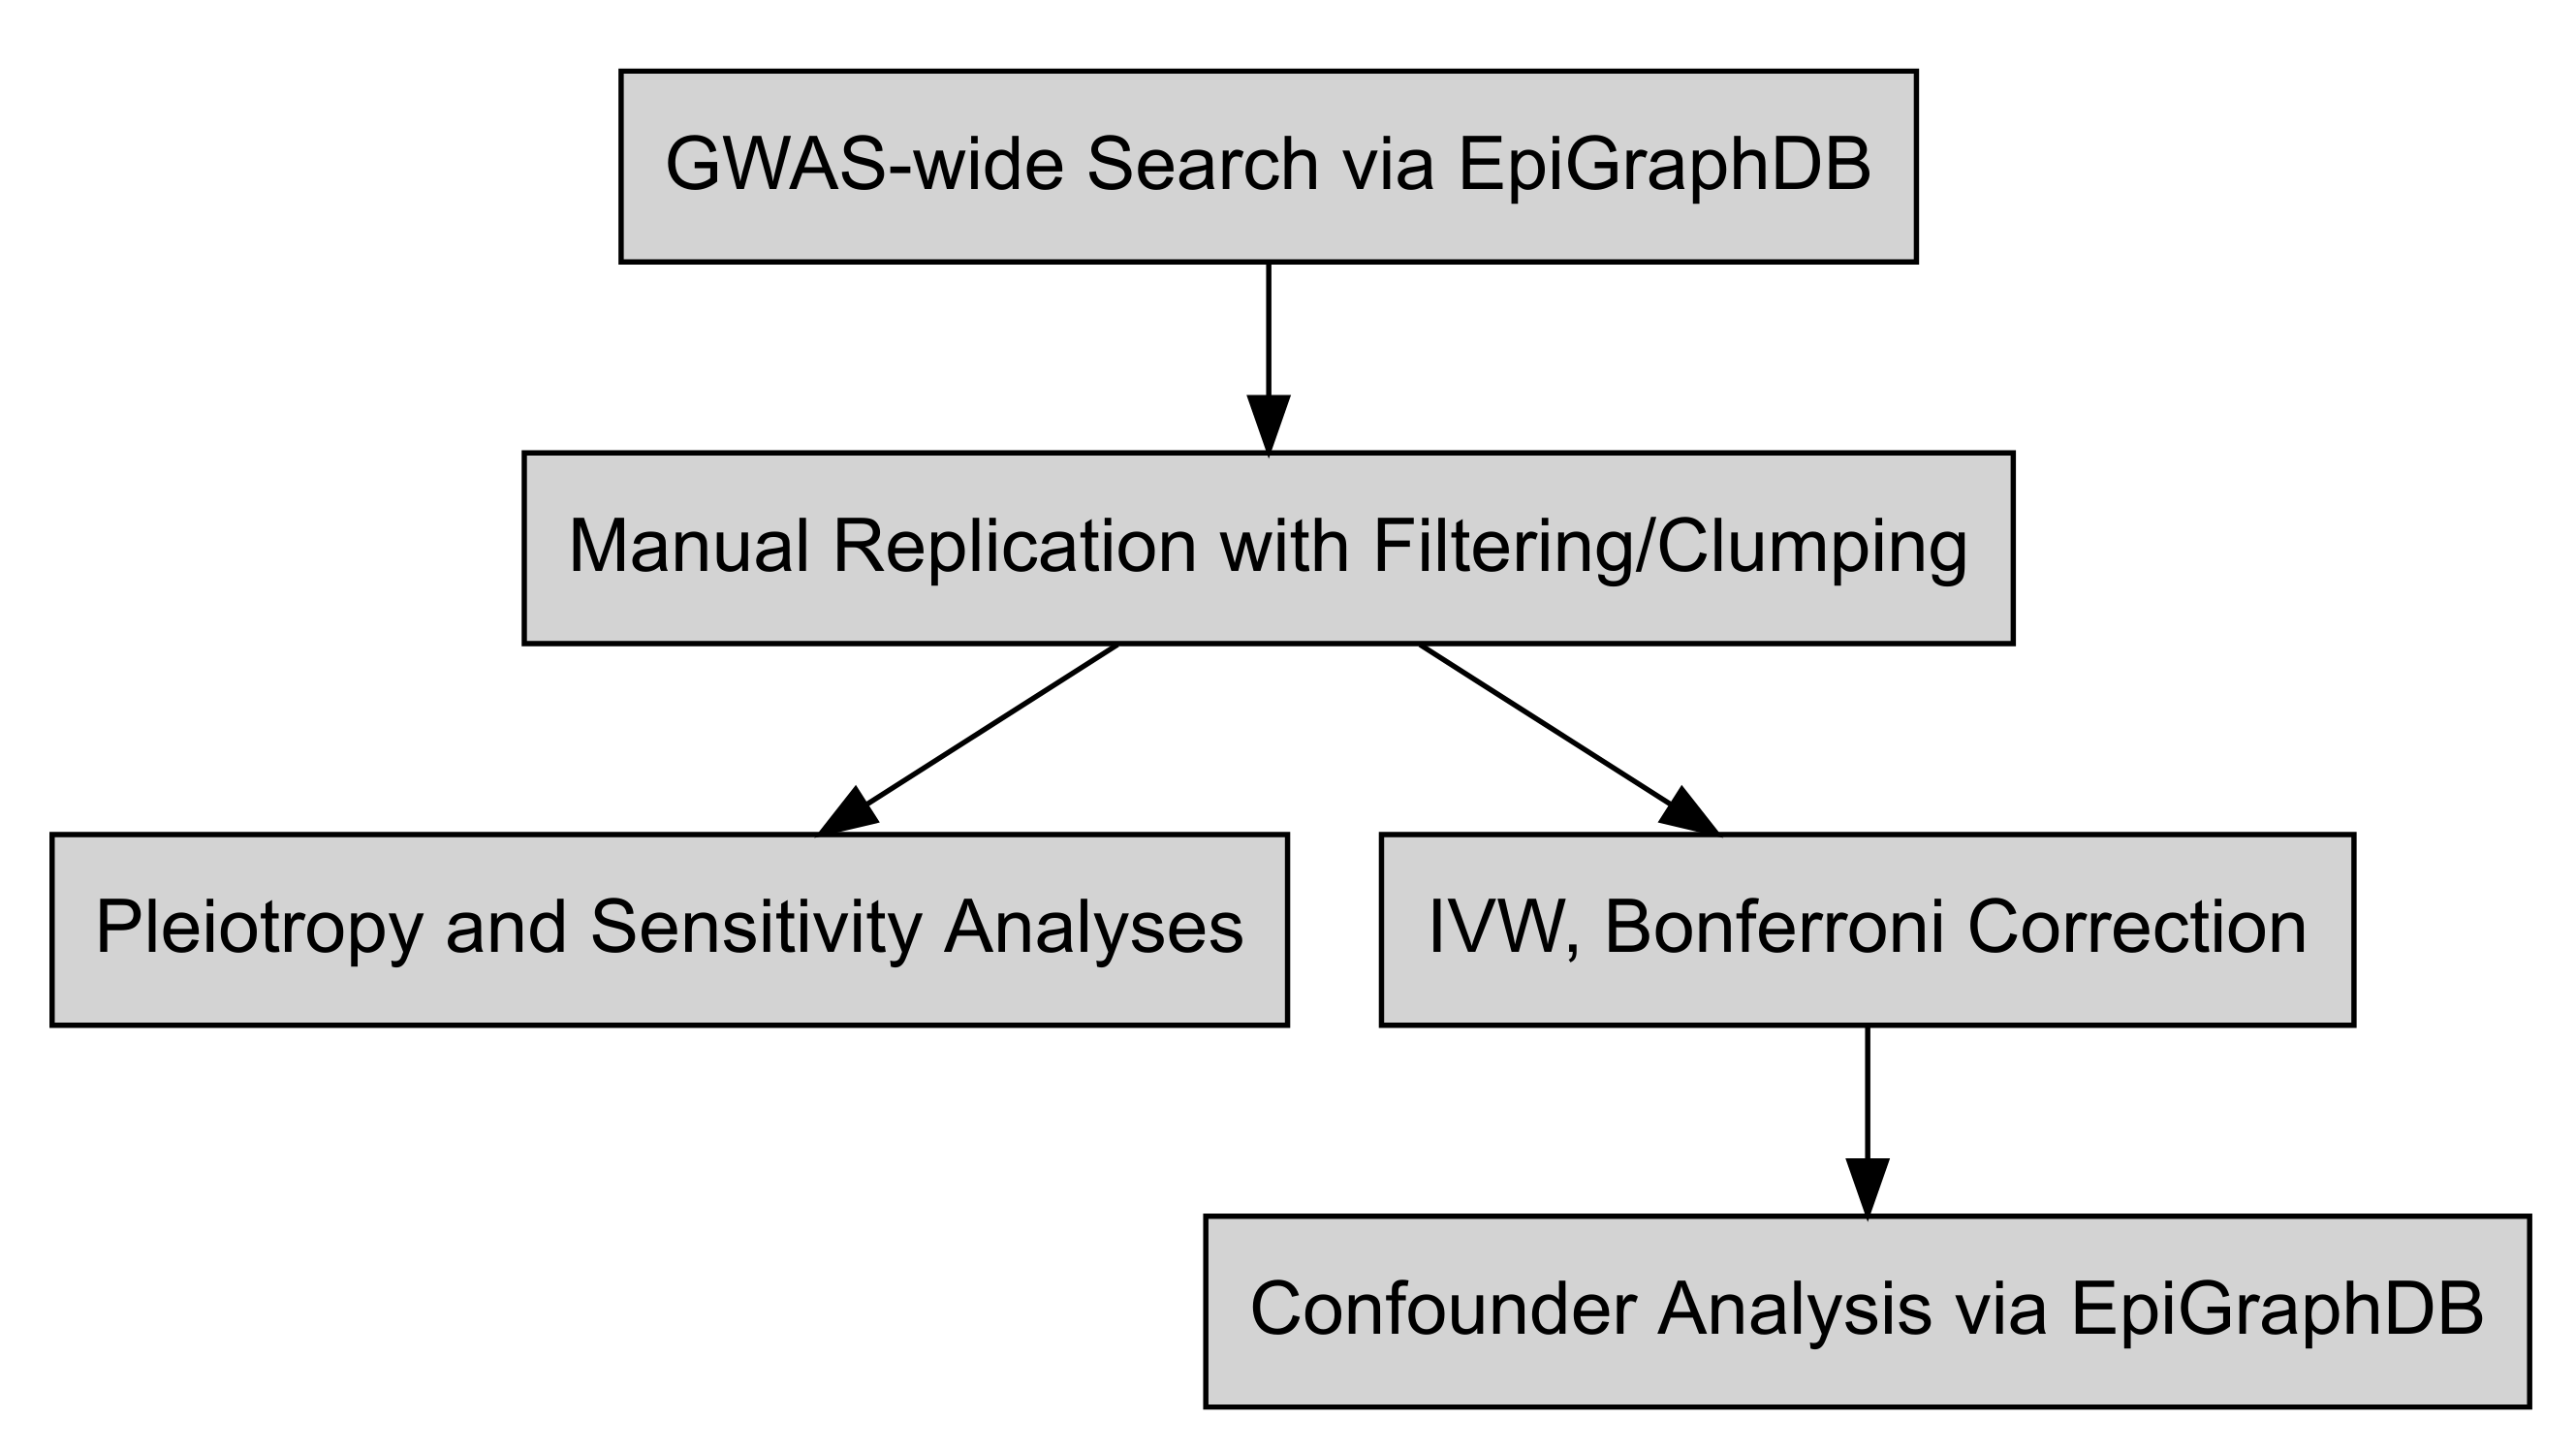
\includegraphics[width=0.9\linewidth]{Figs/Analysis1/outline.png}
	\caption{Mendelian Randomization (MR) workflow for testing the causal influence of chronotype on traits in the EpiGraphDB database. An unbiased search for GWAS-derived two-sample MR studies was performed with chronotype or moningness/eveningness as reported exposures, and IVW results (p < 5e-8) retained. Potential chronotype IVs were processed with Steiger filtering, LD-clumping, and stand/palindromic SNP harmonization. IVW and related MR analyses are then performed on filtered SNP summary statistics, followed by pleiotropy (MR-Egger) and leave-one-out sensitivity analyses. Associations that survive multiple testing correction are then uploaded to EpiGraphDB to investigate potential confounders not present in exposure/trait analyses as reported.}
	\label{fig:MR_Workflow}
\end{figure}

\subsection{Mendelian Randomization Investigations}

Each retained exposure's data was downloaded from MR-Base via TwoSampleMR package version 0.5.5 \cite{hemani_mr-base_2018}. For each instrumental variable (IV) SNP in the exposure study, the following procedure was performed. First, the strandedness of each GWAS was checked to ensure that at each allele, the minor and major alleles were equal. If these were reversed, effect sizes were modified to correct for this. Pallendromic SNPs, which contain alleles represented by the same base pairs on both strands of DNA, were discarded. If SNPs were not present, proxies were found using PLINK with an $R^2$ of at least 0.8, and strand was checked again \cite{plink}. Next, SNPs, in the exposure GWAS set, were clumped by LD to ensure statistical independence. In a window of 10,000 base pairs, an $R^2$ cutoff of < 0.001 was set to obtain haplotype blocks using the European reference panel of the 10,000 Genomes Project \cite{10kgenomes}. In each exposure/outcome pair this left a variable number of SNPs for use as valid, independent IVs (see Figure~\ref{fig:MR_Workflow} top second step). Effect sizes for each SNP were reported as a $\beta$ or the transformed $log(OR)$. The Wald ratio was then obtained, giving a measure of the effect of the exposure on the outcome \cite{rasooly_conducting_2019}: 

\begin{equation}
\widehat{\theta_j}    = \frac{\beta_{Yj}}{\beta_{Xj}}
\end{equation}

where $\beta_Y_j$ is the effect of the IV on the outcome, and $\beta_X_j$ is the effect of the IV on the exposure is obtained for SNP j, and $\widehat{\theta}$ is the effect size.

An initial IVW analysis between each exposure/outcome set was performed, with the false discovery rate (FDR) controlled for \cite{benyamin_family-based_2009}. An FDR of < 0.05 was considered significant. Rather than calculate Wald ratios individually, the outcome GWAS $\beta$s or Odds Ratios are regressed on the exposure in an inverse variance weighted (IVW) meta-analysis. The slope of the regression line indicates the strength of the effect, as an increase in the unit of outcome per unit of the exposure\cite{burgess_interpreting_2017}. 
In a IVW meta-analysis, the  IVW estimate is calculated by:

\begin{equation}
\widehat{\beta}_{Yj} = \theta_{IVW}\widehat{\beta}_{Xj} + \epsilon_{Ij};      \epsilon_{Ij} \sim N(0,\sigma^2se(\widehat{\beta}_{Yj})^2)
\end{equation}

where $\widehat{\theta}$ is the inverse variance weighted average, $se$ is the standard error, I is an error term (Figure~\ref{fig:MR_Workflow} third step, right), and other terms are as above.

Ten significant IVW studies were then subject to four additional MR methods (Figure~\ref{fig:MR_Workflow}, third level left).  To address unseen horizontal pleiotropy, the Egger regression was performed. \cite{bowden_framework_2017,bowdenMendelianRandomizationInvalid2015b}. The Wald ratios of each SNP are used in meta-regression by taking the inverse variance weights used in the IVW analysis without modeling the intercept. As a result, a causal estimate, similar to IVW, is obtained, adjusted though for horizontal pleiotropy which is necessary so as to ensure IVW validity \cite{bowdenMendelianRandomizationInvalid2015b}.
MR-Egger regression is an extension of IVW regression. Instead of assuming no intercept term, an intercept is estimated:
\begin{equation}
\widehat{\beta}_{Yj} = \theta_{0E} + \theta_{1E}\widehat{\beta}_{Xj} + \epsilon_{Ej}; \epsilon_{Ej} \sim N(0,\sigma^2se(\widehat{\beta}_{Yj})^2)
\end{equation}
where $\theta_{0E}$ is the intercept and $\theta_{1E}$ the MR-Egger estimate.
If the intercept is equal to zero, then the IVW method and MR-Egger will be equivalent \cite{burgess_interpreting_2017}. During the IVW process in MR-Egger, the effect sizes of each SNP must have the same sign, and this decreases the variation between them \cite{bowdenMendelianRandomizationInvalid2015b}.

Inverse variance-weighted median analyses were performed, using the median of the Wald ratios as an effect size. Unweighted analyses assume that over half of the instruments are valid, while in a weighted median analysis the assumption is that the at least 50\% of the weight of the instruments are valid themselves \cite{bowden_consistent_2016}. This approach is robust to directional pleiotropy when compared to a simple IVW meta-analysis.

The mode-based estimator (MBE) clusters Wald ratios before calculating random effects in an IVW meta-analysis \cite{hartwigRobustInferenceSummary2017a}. The simple MBE uses unweighted analysis, while the weighted MBE uses inverse variance weighting. First, a smooth empirical density function is calculated for each Wald ratio and are then clustered. The ZEMPA assumption (Zero Modal Pleiotropy Assumption) states that the biggest cluster with the same ratio estimates will be valid instruments. These were used in each analysis, resulting in fewer SNPs and less power, but an increase in potential robustness to horizontal pleiotropy.

Heterogeneity can occur when individual SNPs do not converge on an estimate; this was estimated by Cochran's $Q$ \cite{higgins_cochrane_2011}. In this context, heterogeneity may be a sign of horizontal pleiotropy, wherein SNPs effect the outcome by their influence on other confounding traits \cite{burgess_review_2017}. To inspect SNPs for outliers, we performed leave-one-out sensitivity analyses using the IVW method, leaving out one SNP in each analysis. 

We used the Steiger test to access the directionality of all causative analyses post-hoc \cite{hemaniOrientingCausalRelationship2017}. The Steiger test first assesses which variables (exposure or outcome) are influenced by the SNPs used, by testing if the SNPs explain more variance in the exposure than in the outcome with a modified $Z$ statistic. If the p-value of the IVW estimate and the Steiger estimate are both significant, the sign of the $Z$ statistic is used to assign the correct causal direction between exposure and outcome.

\subsection{Confounder and Intermediate Analysis}
To address potential confounders, not seen in pairwise analyses even in the absence of the statistical suggestion of horizontal pleiotropy, existing MR studies were obtained from EpiGraphDB (Figure~\ref{fig:MR_Workflow} last step). Each study exposure/outcome pair with significant FDR-corrected IVW results was used to interrogate the database for intermediate, reverse intermediate, collider, and confounding variables. Results from the study database surpassing a p-value threshold of < 1e-5, using a fixed effects IVW method only, were retained. The $\beta$ effect sizes for significant results between exposures and outcomes, exposures and confounders, and outcomes and confounders were used to create a weighted directed graph in Cytoscape \cite{shannon_cytoscape_2003} version 3.8.2, and the yFiles Organic (force directed) layout to visualize the relationships between traits. 

All statistical analyses were performed in R version 4.0.5 \cite{r_core_team_r:_2013}. 


%%%%%%%%%%%%%%%%%%%%%%%%%%%%%%%%%%%%%%%%%%

\section{Results}
Initially, 120 prospective studies were identified using EpiGraphDB containing chronotype as an exposure \ref{AllDB_ChronoMRExposure}. Of these, there were 28 primary associations, with IVW p-values of < 5e-8, directly relevant to this study, including measures of alcohol intake, bipolar disorder, T2DM (type 2 diabetes mellitus) as well as testosterone and triglyceride levels. Since the analyses were performed in a high-throughput environment, we re-analyzed each relevant study with the IVW method using summary statistics( Figure~\ref{forestIVW}). Following filtering and quality control, 10 studies held up to a false discovery rate of p < 0.05. The bi-directional nature of the forest plot exists due the different nature of the chronotype exposure studies (treating morning or evening chronotype as case/control). Each of the 10 studies were further analysed with a tendency toward eveningness reflecting a high $\beta$ value in the exposure effect size. 

%% table: traits with genome-wide significance in EpiGraphDB
% latex table generated in R 4.0.5 by xtable 1.8-4 package
% Wed May 12 17:56:06 2021
\begin{table}[ht]
\centering
\begin{tabular}{lllrrr}
  \hline
 & Exposure & Outcome & Beta & SE & P-value \\ 
  \hline
1 & Morning/evening person (chronotype) & Primary biliary cirrhosis & 1.6434941 & 0.0367252 & 0.0000000000 \\ 
  2 & Morning/evening person (chronotype) & Celiac disease & 0.3316132 & 0.0105306 & 0.0000000000 \\ 
  3 & Morning/evening person (chronotype) & CD4mem:\%cFTH (2) & 0.1007642 & 0.0042008 & 0.0000000000 \\ 
  4 & Morning/evening person (chronotype) & CD8:\%TEM & -0.1895340 & 0.0084737 & 0.0000000000 \\ 
  5 & Morning/evening person (chronotype) & Waking too early & -0.1562427 & 0.0165909 & 0.0000000000 \\ 
  6 & Morning/evening person (chronotype) & Narcolepsy & -1.6414641 & 0.1976260 & 0.0000000000 \\ 
  7 & Morning/evening person (chronotype) & Bipolar disorder & 0.1716641 & 0.0249862 & 0.0000000000 \\ 
  8 & Morning/evening person (chronotype) & Waking too early & -0.1333709 & 0.0196971 & 0.0000000000 \\ 
  9 & Morning/evening person (chronotype) & Average weekly beer plus cider intake & 0.0843970 & 0.0127507 & 0.0000000000 \\ 
  10 & Morning/evening person (chronotype) & Juvenile idiopathic arthritis (oligoarticular or rheumatoid factor-negative polyarticular) & 2.2616377 & 0.3440739 & 0.0000000000 \\ 
  11 & Morning/evening person (chronotype) & Victim of physically violent crime & 0.0524804 & 0.0080605 & 0.0000000001 \\ 
  12 & Morning/evening person (chronotype) & Sleeping too much & 0.1098961 & 0.0184369 & 0.0000000025 \\ 
  13 & Morning/evening person (chronotype) & Blood clot, DVT, bronchitis, emphysema, asthma, rhinitis, eczema, allergy diagnosed by doctor: Hayfever, allergic rhinitis or eczema & 0.0296773 & 0.0050327 & 0.0000000037 \\ 
  14 & Morning/evening person (chronotype) & Lifetime number of sexual partners & 0.0749294 & 0.0127072 & 0.0000000037 \\ 
  15 & Morning/evening person (chronotype) & Lymph:\%NK & -0.2424444 & 0.0429612 & 0.0000000167 \\ 
  16 & Morning/evening person (chronotype) & Frequency of tiredness / lethargy in last 2 weeks & 0.0670919 & 0.0119551 & 0.0000000200 \\ 
  17 & Morning/evening person (chronotype) & Ulcerative colitis & 0.6925179 & 0.1238467 & 0.0000000225 \\ 
  18 & Morning/evening person (chronotype) & Ulcerative colitis & 0.6925179 & 0.1238467 & 0.0000000225 \\ 
  19 & Chronotype & Levulinate (4-oxovalerate) & -0.0695406 & 0.0004251 & 0.0000000000 \\ 
  20 & Chronotype & Levulinate (4-oxovalerate) & -0.0695406 & 0.0004251 & 0.0000000000 \\ 
  21 & Chronotype & Subjective well-being & -0.2105027 & 0.0076672 & 0.0000000000 \\ 
  22 & Chronotype & Subjective well-being & -0.2105027 & 0.0076672 & 0.0000000000 \\ 
  23 & Chronotype & X-14205--alpha-glutamyltyrosine & -0.1342457 & 0.0062338 & 0.0000000000 \\ 
  24 & Chronotype & X-14205--alpha-glutamyltyrosine & -0.1342457 & 0.0062338 & 0.0000000000 \\ 
  25 & Chronotype & Tryptophan betaine & 0.4708220 & 0.0237419 & 0.0000000000 \\ 
  26 & Chronotype & Tryptophan betaine & 0.4708220 & 0.0237419 & 0.0000000000 \\ 
  27 & Chronotype & Ulcerative colitis & 0.4487501 & 0.0228454 & 0.0000000000 \\ 
  28 & Chronotype & Ulcerative colitis & 0.4487501 & 0.0228454 & 0.0000000000 \\ 
  29 & Chronotype & X-12510--2-aminooctanoic acid & 0.0842249 & 0.0044018 & 0.0000000000 \\ 
  30 & Chronotype & X-12510--2-aminooctanoic acid & 0.0842249 & 0.0044018 & 0.0000000000 \\ 
  31 & Chronotype & PCT responsible for patient data: RICHMOND AND TWICKENHAM PCT & 0.0055308 & 0.0003863 & 0.0000000000 \\ 
  32 & Chronotype & PCT responsible for patient data: RICHMOND AND TWICKENHAM PCT & 0.0055308 & 0.0003863 & 0.0000000000 \\ 
  33 & Chronotype & PCT where patients GP was registered: TRAFFORD NORTH PCT & -0.0041719 & 0.0003006 & 0.0000000000 \\ 
  34 & Chronotype & PCT where patients GP was registered: TRAFFORD NORTH PCT & -0.0041719 & 0.0003006 & 0.0000000000 \\ 
  35 & Chronotype & Diagnoses - main ICD10: Z42.1 Follow-up care involving plastic surgery of breast & -0.0043565 & 0.0003525 & 0.0000000000 \\ 
  36 & Chronotype & Diagnoses - main ICD10: Z42.1 Follow-up care involving plastic surgery of breast & -0.0043565 & 0.0003525 & 0.0000000000 \\ 
  37 & Chronotype & X-12094 & -0.1048936 & 0.0096090 & 0.0000000000 \\ 
  38 & Chronotype & X-12094 & -0.1048936 & 0.0096090 & 0.0000000000 \\ 
  39 & Chronotype & Diagnoses - secondary ICD10: Z86.1 Personal history of infectious and parasitic diseases & -0.0037513 & 0.0003674 & 0.0000000000 \\ 
  40 & Chronotype & Diagnoses - secondary ICD10: Z86.1 Personal history of infectious and parasitic diseases & -0.0037513 & 0.0003674 & 0.0000000000 \\ 
  41 & Chronotype & X-11552 & 0.0314310 & 0.0032494 & 0.0000000000 \\ 
  42 & Chronotype & X-11552 & 0.0314310 & 0.0032494 & 0.0000000000 \\ 
  43 & Chronotype & Diagnoses - secondary ICD10: M47.82 Other spondylosis (Cervical region) & -0.0047349 & 0.0005081 & 0.0000000000 \\ 
  44 & Chronotype & Diagnoses - secondary ICD10: M47.82 Other spondylosis (Cervical region) & -0.0047349 & 0.0005081 & 0.0000000000 \\ 
  45 & Chronotype & X-12244--N-acetylcarnosine & -0.0980723 & 0.0112319 & 0.0000000000 \\ 
  46 & Chronotype & X-12244--N-acetylcarnosine & -0.0980723 & 0.0112319 & 0.0000000000 \\ 
  47 & Chronotype & Bilirubin (Z,Z) & 0.1330162 & 0.0152930 & 0.0000000000 \\ 
  48 & Chronotype & Bilirubin (Z,Z) & 0.1330162 & 0.0152930 & 0.0000000000 \\ 
  49 & Chronotype & Type 2 diabetes & 0.8268623 & 0.0994853 & 0.0000000000 \\ 
  50 & Chronotype & Type 2 diabetes & 0.8268623 & 0.0994853 & 0.0000000000 \\ 
  51 & Chronotype & X-11521 & 0.1554129 & 0.0188887 & 0.0000000000 \\ 
  52 & Chronotype & X-11521 & 0.1554129 & 0.0188887 & 0.0000000000 \\ 
  53 & Chronotype & X-12847 & 0.1760735 & 0.0219797 & 0.0000000000 \\ 
  54 & Chronotype & X-12847 & 0.1760735 & 0.0219797 & 0.0000000000 \\ 
  55 & Chronotype & Operative procedures - secondary OPCS: S57.1 Debridement of skin NEC & 0.0041534 & 0.0005233 & 0.0000000000 \\ 
  56 & Chronotype & Operative procedures - secondary OPCS: S57.1 Debridement of skin NEC & 0.0041534 & 0.0005233 & 0.0000000000 \\ 
  57 & Chronotype & Operative procedures - main OPCS: M47.4 Urodynamic studies using catheter & 0.0019398 & 0.0002456 & 0.0000000000 \\ 
  58 & Chronotype & Operative procedures - main OPCS: M47.4 Urodynamic studies using catheter & 0.0019398 & 0.0002456 & 0.0000000000 \\ 
  59 & Chronotype & Type 2 diabetes & 0.4708763 & 0.0600415 & 0.0000000000 \\ 
  60 & Chronotype & Type 2 diabetes & 0.4708763 & 0.0600415 & 0.0000000000 \\ 
  61 & Chronotype & Treatment/medication code: nicorandil & -0.0074871 & 0.0009831 & 0.0000000000 \\ 
  62 & Chronotype & Treatment/medication code: nicorandil & -0.0074871 & 0.0009831 & 0.0000000000 \\ 
  63 & Chronotype & Type 2 diabetes & 0.4815483 & 0.0650125 & 0.0000000000 \\ 
  64 & Chronotype & Type 2 diabetes & 0.4815483 & 0.0650125 & 0.0000000000 \\ 
  65 & Chronotype & Omega-3 fatty acids & 0.6280975 & 0.0852501 & 0.0000000000 \\ 
  66 & Chronotype & Omega-3 fatty acids & 0.6280975 & 0.0852501 & 0.0000000000 \\ 
  67 & Chronotype & X-11850 & 0.2931782 & 0.0411490 & 0.0000000000 \\ 
  68 & Chronotype & X-11850 & 0.2931782 & 0.0411490 & 0.0000000000 \\ 
  69 & Chronotype & 4-methyl-2-oxopentanoate & -0.1106728 & 0.0159103 & 0.0000000000 \\ 
  70 & Chronotype & 4-methyl-2-oxopentanoate & -0.1106728 & 0.0159103 & 0.0000000000 \\ 
  71 & Chronotype & Sources of admission to hospital (recoded): Transfer within NHS provider: Surgical specialty & 0.0037020 & 0.0005628 & 0.0000000000 \\ 
  72 & Chronotype & Sources of admission to hospital (recoded): Transfer within NHS provider: Surgical specialty & 0.0037020 & 0.0005628 & 0.0000000000 \\ 
  73 & Chronotype & Treatment/medication code: alfuzosin & -0.0028755 & 0.0004477 & 0.0000000001 \\ 
  74 & Chronotype & Treatment/medication code: alfuzosin & -0.0028755 & 0.0004477 & 0.0000000001 \\ 
  75 & Chronotype & X-14632 & 0.0920730 & 0.0143633 & 0.0000000001 \\ 
  76 & Chronotype & X-14632 & 0.0920730 & 0.0143633 & 0.0000000001 \\ 
  77 & Chronotype & Diagnoses - main ICD10: D17.2 Benign lipomatous neoplasm of skin and subcutaneous tissue of limbs & -0.0052601 & 0.0008339 & 0.0000000003 \\ 
  78 & Chronotype & Diagnoses - main ICD10: D17.2 Benign lipomatous neoplasm of skin and subcutaneous tissue of limbs & -0.0052601 & 0.0008339 & 0.0000000003 \\ 
  79 & Chronotype & Chondroitin sulfate proteoglycan 4 & -0.4517760 & 0.0742204 & 0.0000000012 \\ 
  80 & Chronotype & Testosterone levels & -0.2971242 & 0.0488982 & 0.0000000012 \\ 
  81 & Chronotype & Testosterone levels & -0.2971242 & 0.0488982 & 0.0000000012 \\ 
  82 & Chronotype & IDP dMRI TBSS L3 Anterior corona radiata R & 0.3172729 & 0.0527558 & 0.0000000018 \\ 
  83 & Chronotype & IDP dMRI TBSS L3 Anterior corona radiata R & 0.3172729 & 0.0527558 & 0.0000000018 \\ 
  84 & Chronotype & Diagnoses - main ICD10: N20 Calculus of kidney and ureter & 0.0065320 & 0.0010871 & 0.0000000019 \\ 
  85 & Chronotype & Diagnoses - main ICD10: N20 Calculus of kidney and ureter & 0.0065320 & 0.0010871 & 0.0000000019 \\ 
  86 & Chronotype & X-12524 & -0.0657029 & 0.0109883 & 0.0000000022 \\ 
  87 & Chronotype & X-12524 & -0.0657029 & 0.0109883 & 0.0000000022 \\ 
  88 & Chronotype & Omega-7, omega-9 and saturated fatty acids & 0.5807043 & 0.0972531 & 0.0000000024 \\ 
  89 & Chronotype & Omega-7, omega-9 and saturated fatty acids & 0.5807043 & 0.0972531 & 0.0000000024 \\ 
  90 & Chronotype & Serine/threonine-protein kinase pim-1 & 0.4629941 & 0.0781389 & 0.0000000031 \\ 
  91 & Chronotype & Triglycerides & -0.1639666 & 0.0276901 & 0.0000000032 \\ 
  92 & Chronotype & Triglycerides & -0.1639666 & 0.0276901 & 0.0000000032 \\ 
  93 & Chronotype & Triglycerides & -0.1639666 & 0.0276901 & 0.0000000032 \\ 
  94 & Chronotype & Triglycerides & -0.1639666 & 0.0276901 & 0.0000000032 \\ 
  95 & Chronotype & Getting up in morning & 0.2470261 & 0.0417617 & 0.0000000033 \\ 
  96 & Chronotype & Getting up in morning & 0.2470261 & 0.0417617 & 0.0000000033 \\ 
  97 & Chronotype & Treatment/medication code: calcium salts & 0.0101307 & 0.0017271 & 0.0000000045 \\ 
  98 & Chronotype & Treatment/medication code: calcium salts & 0.0101307 & 0.0017271 & 0.0000000045 \\ 
  99 & Chronotype & Operative procedures - secondary OPCS: S06.9 Unspecified other excision of lesion of skin & -0.0076851 & 0.0013104 & 0.0000000045 \\ 
  100 & Chronotype & Operative procedures - secondary OPCS: S06.9 Unspecified other excision of lesion of skin & -0.0076851 & 0.0013104 & 0.0000000045 \\ 
  101 & Chronotype & PCT responsible for patient data: BARNSLEY PCT & -0.0038987 & 0.0006654 & 0.0000000046 \\ 
  102 & Chronotype & PCT responsible for patient data: BARNSLEY PCT & -0.0038987 & 0.0006654 & 0.0000000046 \\ 
  103 & Chronotype & Operative procedures - secondary OPCS: U08.1 Computed tomography of abdomen NEC & -0.0028017 & 0.0004790 & 0.0000000049 \\ 
  104 & Chronotype & Operative procedures - secondary OPCS: U08.1 Computed tomography of abdomen NEC & -0.0028017 & 0.0004790 & 0.0000000049 \\ 
  105 & Chronotype & Rotator cuff syndrome & 0.0086883 & 0.0015019 & 0.0000000073 \\ 
  106 & Chronotype & Rotator cuff syndrome & 0.0086883 & 0.0015019 & 0.0000000073 \\ 
  107 & Chronotype & Total fatty acids & 0.6218546 & 0.1079104 & 0.0000000083 \\ 
  108 & Chronotype & Total fatty acids & 0.6218546 & 0.1079104 & 0.0000000083 \\ 
  109 & Chronotype & Diagnoses - secondary ICD10: K51.9 Ulcerative colitis, unspecified & 0.0048540 & 0.0008598 & 0.0000000165 \\ 
  110 & Chronotype & Diagnoses - secondary ICD10: K51.9 Ulcerative colitis, unspecified & 0.0048540 & 0.0008598 & 0.0000000165 \\ 
  111 & Chronotype & Serum total triglycerides & 0.3627431 & 0.0643037 & 0.0000000169 \\ 
  112 & Chronotype & Serum total triglycerides & 0.3627431 & 0.0643037 & 0.0000000169 \\ 
  113 & Chronotype & Illnesses of mother: High blood pressure & 0.0448683 & 0.0079776 & 0.0000000186 \\ 
  114 & Chronotype & Illnesses of mother: High blood pressure & 0.0448683 & 0.0079776 & 0.0000000186 \\ 
  115 & Chronotype & Operative procedures - main OPCS: F09.5 Surgical removal of retained root of tooth & 0.0039863 & 0.0007118 & 0.0000000214 \\ 
  116 & Chronotype & Operative procedures - main OPCS: F09.5 Surgical removal of retained root of tooth & 0.0039863 & 0.0007118 & 0.0000000214 \\ 
  117 & Chronotype & N2,N2-dimethylguanosine & -0.0566029 & 0.0102502 & 0.0000000335 \\ 
  118 & Chronotype & N2,N2-dimethylguanosine & -0.0566029 & 0.0102502 & 0.0000000335 \\ 
  119 & Chronotype & NET100 0870 & 0.6264433 & 0.1143457 & 0.0000000429 \\ 
  120 & Chronotype & NET100 0870 & 0.6264433 & 0.1143457 & 0.0000000429 \\ 
   \hline
\end{tabular}
\caption{Causal associations resulting from exposure to chronotype mined from EpiGraphDB. SE = standard error.} 
\label{AllDB_ChronoMRExposure}
\end{table}

%% figure: re-analysis forest plots of significant traits
\begin{figure}[htbp]
	\centering
	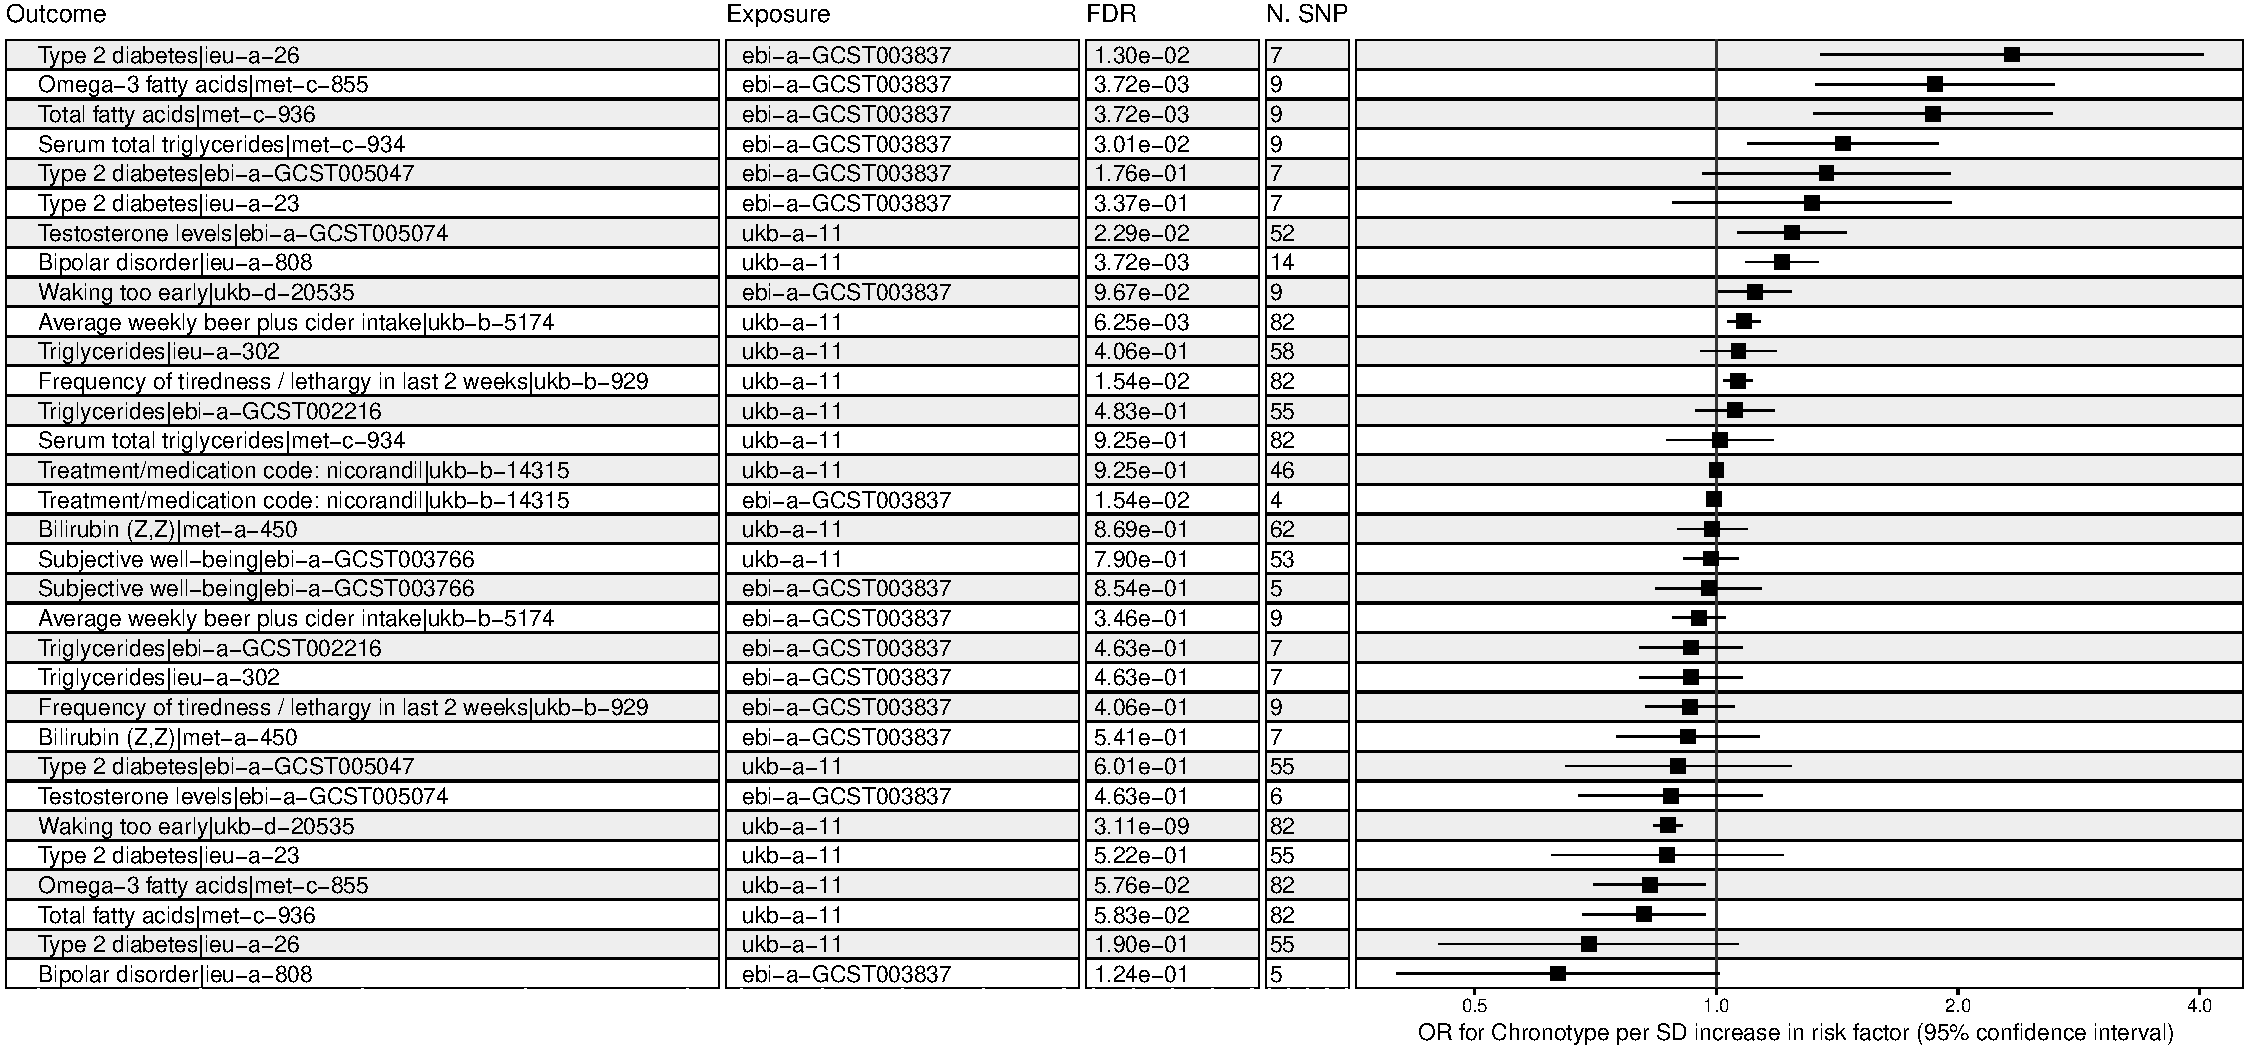
\includegraphics[width=\linewidth]{Figs/Analysis1/forestIVW1a.pdf}
	\caption{Causal relationships between exposure to chronotype and various traits. Causal associations mined from EpiGraphDB (IVW p < 5e-8) were analyzed using two chronotype exposure measures. Outcomes are listed with trait and study accession number. Exposure \textit{ebi-a-GCST003837} reflects SD increase in chronotype on a continuous morning - evening scale. Exposure \textit{ukb-a-11} represents odds of an evening chronotype. Effect sizes are from fixed-effects inverse variance weighted analyses with 95\% confidence intervals. False discovery rate-corrected p-values are shown.}
	\label{forestIVW}
\end{figure}

\subsection{Chronotype influences on diabetes, alcohol consumption, and bipolar disorder}
The strongest associations ($\beta$ > 0.90) include risk for T2DM and total fatty acid concentration. T2DM included 7 independent SNPs, see Supplemental Table~\ref{FDR_Signif_CHR_Exposure}. The weakest association was with the MR-Egger method, $\beta$ = 0.73, which while not highly significant (p = 0.04) did not reveal evidence of horizontal pleiotropy (intercept p-value = 0.98) or heterogeneity (Egger Q p-value 0.99). The IVW analysis and weighted median analysis each concurred (p = 0.002 and 0.009), suggesting little loss of associative signal even if some of the 7 SNPs were biased by pleiotropy. Leave one out sensitivity analyses suggests that no one IV dominates the model, and all methods have similar effect sizes as judged by slope, Figure~\ref{t2dm}. 
% T2DM
\begin{figure}[htbp]
	\centering
         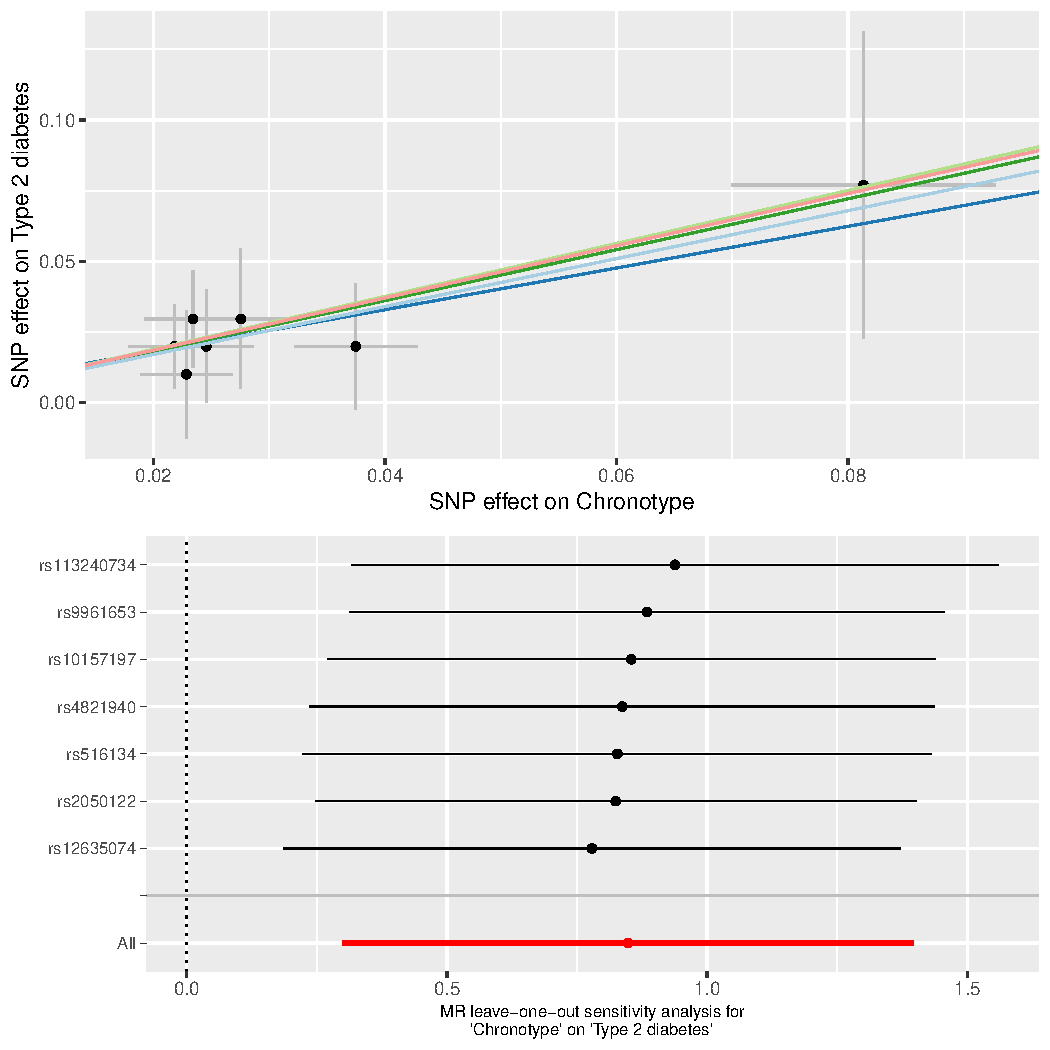
\includegraphics[width=0.7\textwidth]{Figs/Analysis2/Chronotype_vs_Type_2_diabetes.Plots.pdf}
    \caption{An evening chronotype causes increased odds of a type 2 diabetes mellitus diagnosis. IVW, Weighted median, mode, weighted mode, and Egger regressions shown. Lower panel depicts leave-one-out sensitivity analyses with the IVW method.}
	\label{t2dm}
\end{figure}

Chronotype has a weaker but more statistically significant association with the amount of alcoholic beer or cider drinks consumed weekly, with the increase reflected in pints per week consumed (mean among all respondents of 3/week). With an MR-Egger intercept p-value of 0.31 and a significant Egger regression coefficient (p-value = 0.04), the initial analysis provides strong evidence that the trait may not be subject to horizontal pleiotropy. The weighted median and IVW method were again strongest ($\beta$ = 0.089 and 0.79, p = 4.4e-6 and 9.7e-4). There was, however, evidence among the 82 SNPs which passed the threshold for strong heterogeneity (Cochran Q = 333), suggesting pleiotropy or moderating factors for further investigation even in the absence of such suggestions from the MR-Egger intercept significance test. Heterogeneity among SNPs can be observed in Figure~\ref{beer}, while the leave one out analysis shows overlapping confidence intervals in each iteration, suggesting homogeneity on the whole.

% beer
\begin{figure}[htbp]
	\centering
         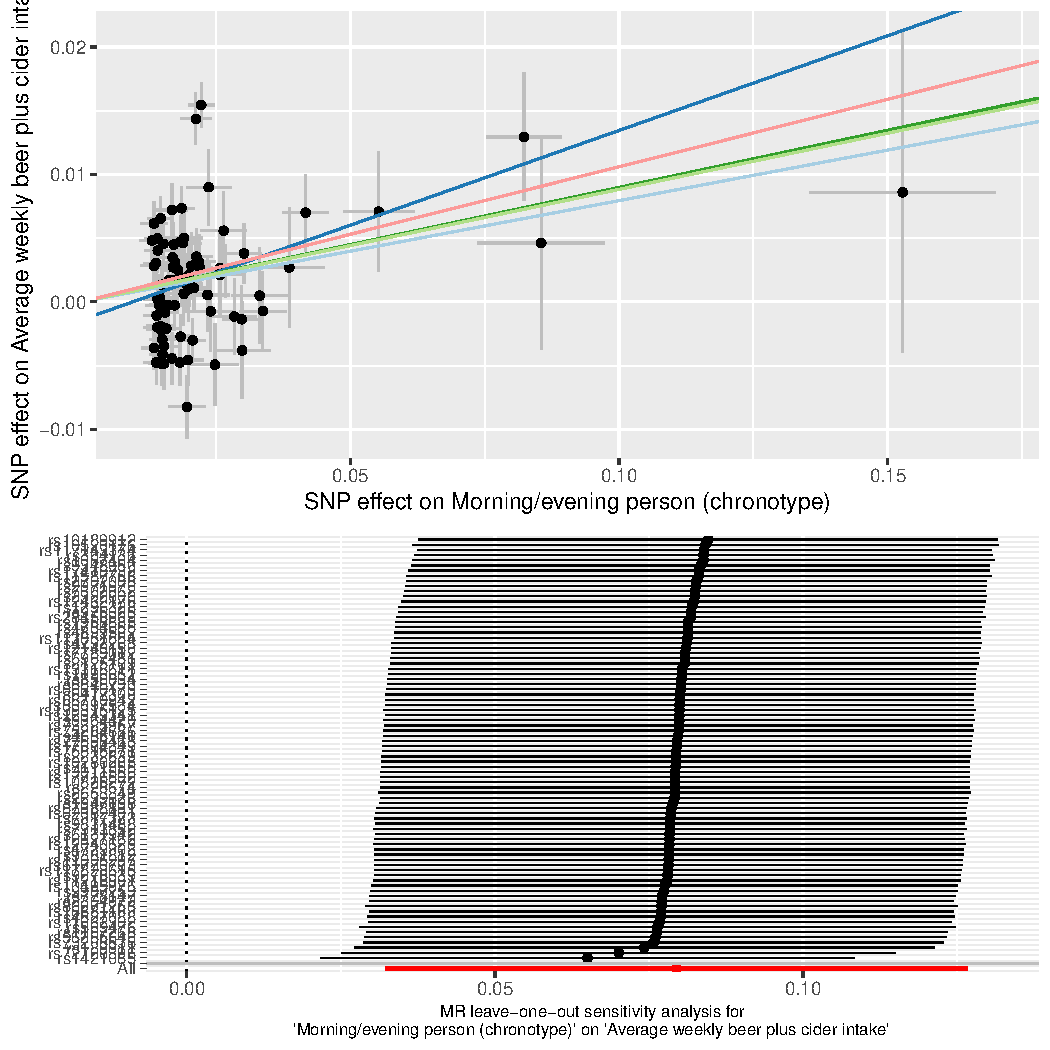
\includegraphics[width=0.7\textwidth]{Figs/Analysis2/Morning_evening_person_(chronotype)_vs_Average_weekly_beer_plus_cider_intake.Plots.pdf}
    \caption{An evening chronotype causes weekly (alcoholic) beer and/or cider intake. IVW, Weighted median, mode, weighted mode, and Egger regressions shown. Lower panel depicts leave-one-out sensitivity analyses with the IVW method.}
	\label{beer}
\end{figure}

The influence of chronotype on bipolar disorder appears substantially varied, with different SNPs with large standard errors apparent in Figure~\ref{bipolar}. The Cochran's Q statistic (Q = 149, p= 2e-24) echoes the visible heterogeneity of SNPs in the analysis. Nevertheless, there is a consistent $\beta$ effect size among the IVW, weighted median, and weighted mode analyses (0.188, 0.175, and 0.181) with are highly statistically significant (p = 4e-4, 1e-11, and 3e-6 respectively). This presents a small but powerful signal that an evening chronotype leads to an increase in activation of pathways leading to bipolar disorder. The test for horizontal pleiotropy, in contrast to the Q statistic, does not suggest horizontal pleiotropy (p = 0.47).

% bipolar
\begin{figure}[htbp]
	\centering
    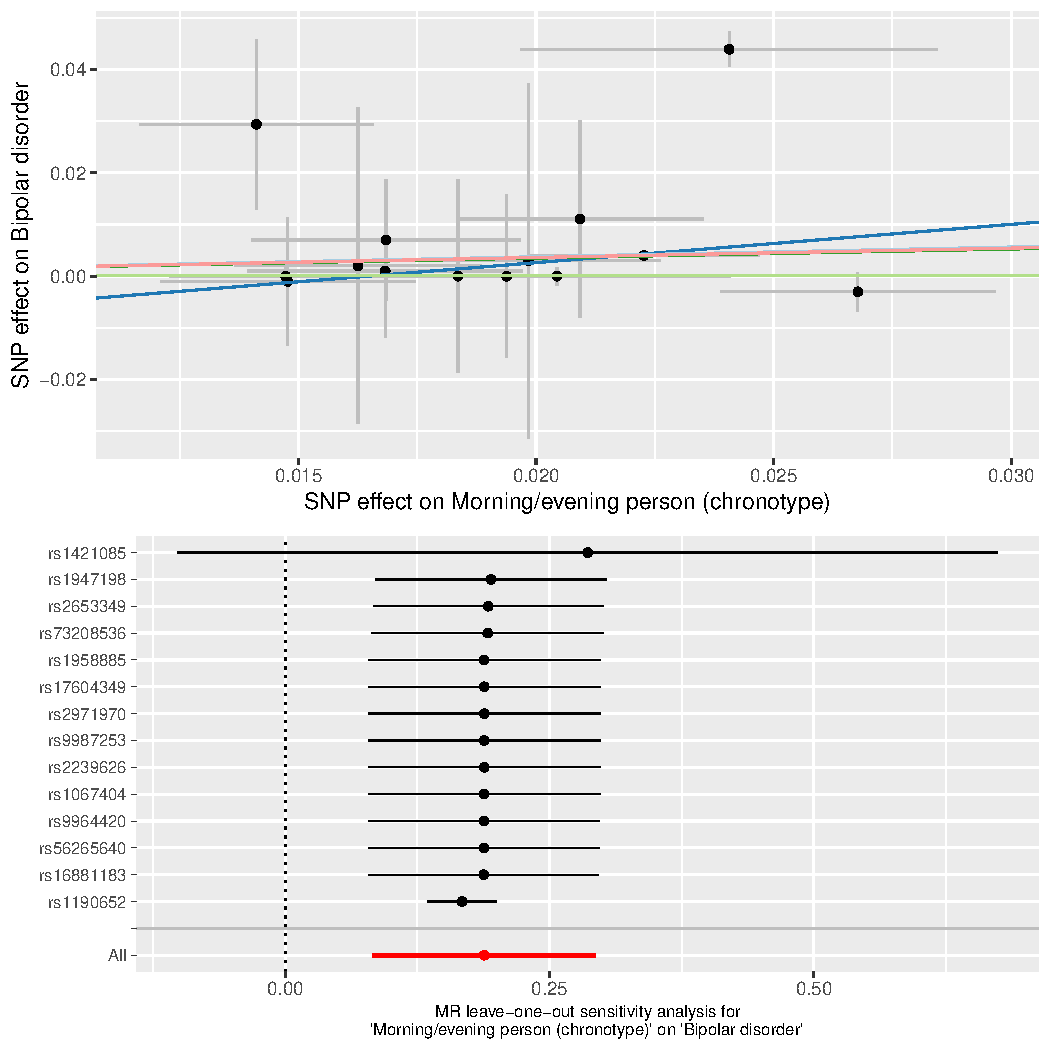
\includegraphics[width=0.7\textwidth]{Figs/Analysis2/Morning_evening_person_(chronotype)_vs_Bipolar_disorder.Plots.pdf}
    \caption{An evening chronotype contributes to the likelihood of a bipolar disorder diagnosis. IVW, Weighted median, mode, weighted mode, and Egger regressions shown. Lower panel depicts leave-one-out sensitivity analyses with the IVW method.}
	\label{bipolar}
\end{figure}

Results for other 7 individual analyses are given in the supplemental materials.
% latex table generated in R 4.0.5 by xtable 1.8-4 package
% Wed May 12 17:58:41 2021
\begin{table}[ht]
\centering
\begin{tabular}{llllllrrrrrrrrrr}
  \hline
 & id.exposure & id.outcome & outcome & exposure & method & nsnp & b & se & pval & Q & Q\_df & Q\_pval & egger\_intercept & intercept\_se & intercept\_pval \\ 
  \hline
1 & ukb-a-11 & ukb-b-929 & Frequency of tiredness / lethargy in last 2 weeks & Morning/evening person (chronotype) & MR Egger & 82 & -0.0295780 & 0.0624363 & 0.6369818 & 237.3310284 & 80 & 0.0000000 & 0.0018546 & 0.001206191 & 0.1281038 \\ 
  2 & ukb-a-11 & ukb-b-929 & Frequency of tiredness / lethargy in last 2 weeks & Morning/evening person (chronotype) & Weighted median & 82 & 0.0663046 & 0.0206812 & 0.0013458 &  &  &  &  &  &  \\ 
  3 & ukb-a-11 & ukb-b-929 & Frequency of tiredness / lethargy in last 2 weeks & Morning/evening person (chronotype) & Inverse variance weighted & 82 & 0.0609076 & 0.0210297 & 0.0037764 & 244.3443707 & 81 & 0.0000000 &  &  &  \\ 
  4 & ukb-a-11 & ukb-b-929 & Frequency of tiredness / lethargy in last 2 weeks & Morning/evening person (chronotype) & Simple mode & 82 & 0.0913902 & 0.0535565 & 0.0917604 &  &  &  &  &  &  \\ 
  5 & ukb-a-11 & ukb-b-929 & Frequency of tiredness / lethargy in last 2 weeks & Morning/evening person (chronotype) & Weighted mode & 82 & 0.0942217 & 0.0584259 & 0.1107056 &  &  &  &  &  &  \\ 
  6 & ukb-a-11 & ukb-d-20535 & Waking too early & Morning/evening person (chronotype) & MR Egger & 82 & -0.2198179 & 0.0640031 & 0.0009435 & 93.4273685 & 80 & 0.1447120 & 0.0016619 & 0.001235910 & 0.1825279 \\ 
  7 & ukb-a-11 & ukb-d-20535 & Waking too early & Morning/evening person (chronotype) & Weighted median & 82 & -0.1315969 & 0.0283806 & 0.0000035 &  &  &  &  &  &  \\ 
  8 & ukb-a-11 & ukb-d-20535 & Waking too early & Morning/evening person (chronotype) & Inverse variance weighted & 82 & -0.1386709 & 0.0214295 & 0.0000000 & 95.5390270 & 81 & 0.1288201 &  &  &  \\ 
  9 & ukb-a-11 & ukb-d-20535 & Waking too early & Morning/evening person (chronotype) & Simple mode & 82 & -0.1031377 & 0.0786971 & 0.1937085 &  &  &  &  &  &  \\ 
  10 & ukb-a-11 & ukb-d-20535 & Waking too early & Morning/evening person (chronotype) & Weighted mode & 82 & -0.1141146 & 0.0800877 & 0.1580367 &  &  &  &  &  &  \\ 
  11 & ukb-a-11 & ebi-a-GCST005074 & Testosterone levels & Morning/evening person (chronotype) & MR Egger & 52 & 0.3530194 & 0.2191494 & 0.1135055 & 58.4597616 & 50 & 0.1926091 & -0.0030082 & 0.004528336 & 0.5095520 \\ 
  12 & ukb-a-11 & ebi-a-GCST005074 & Testosterone levels & Morning/evening person (chronotype) & Weighted median & 52 & 0.3938689 & 0.1140942 & 0.0005562 &  &  &  &  &  &  \\ 
  13 & ukb-a-11 & ebi-a-GCST005074 & Testosterone levels & Morning/evening person (chronotype) & Inverse variance weighted & 52 & 0.2175681 & 0.0798743 & 0.0064520 & 58.9757172 & 51 & 0.2069098 &  &  &  \\ 
  14 & ukb-a-11 & ebi-a-GCST005074 & Testosterone levels & Morning/evening person (chronotype) & Simple mode & 52 & 0.5640466 & 0.2611287 & 0.0354936 &  &  &  &  &  &  \\ 
  15 & ukb-a-11 & ebi-a-GCST005074 & Testosterone levels & Morning/evening person (chronotype) & Weighted mode & 52 & 0.4992242 & 0.2452166 & 0.0469759 &  &  &  &  &  &  \\ 
  16 & ebi-a-GCST003837 & ieu-a-26 & Type 2 diabetes & Chronotype & MR Egger & 7 & 0.7379009 & 0.8374158 & 0.4185654 & 0.8492935 & 5 & 0.9737833 & 0.0032934 & 0.023506006 & 0.8940423 \\ 
  17 & ebi-a-GCST003837 & ieu-a-26 & Type 2 diabetes & Chronotype & Weighted median & 7 & 0.9010107 & 0.3487253 & 0.0097739 &  &  &  &  &  &  \\ 
  18 & ebi-a-GCST003837 & ieu-a-26 & Type 2 diabetes & Chronotype & Inverse variance weighted & 7 & 0.8484831 & 0.2799008 & 0.0024345 & 0.8689243 & 6 & 0.9900970 &  &  &  \\ 
  19 & ebi-a-GCST003837 & ieu-a-26 & Type 2 diabetes & Chronotype & Simple mode & 7 & 0.9377698 & 0.4514314 & 0.0830415 &  &  &  &  &  &  \\ 
  20 & ebi-a-GCST003837 & ieu-a-26 & Type 2 diabetes & Chronotype & Weighted mode & 7 & 0.9242767 & 0.4199526 & 0.0700146 &  &  &  &  &  &  \\ 
  21 & ukb-a-11 & ieu-a-808 & Bipolar disorder & Morning/evening person (chronotype) & MR Egger & 14 & 0.7404360 & 0.7537317 & 0.3453144 & 142.9844543 & 12 & 0.0000000 & -0.0121835 & 0.016582844 & 0.4766326 \\ 
  22 & ukb-a-11 & ieu-a-808 & Bipolar disorder & Morning/evening person (chronotype) & Weighted median & 14 & 0.1752023 & 0.0259165 & 0.0000000 &  &  &  &  &  &  \\ 
  23 & ukb-a-11 & ieu-a-808 & Bipolar disorder & Morning/evening person (chronotype) & Inverse variance weighted & 14 & 0.1881280 & 0.0537517 & 0.0004653 & 149.4162527 & 13 & 0.0000000 &  &  &  \\ 
  24 & ukb-a-11 & ieu-a-808 & Bipolar disorder & Morning/evening person (chronotype) & Simple mode & 14 & 0.0064820 & 0.1191680 & 0.9574486 &  &  &  &  &  &  \\ 
  25 & ukb-a-11 & ieu-a-808 & Bipolar disorder & Morning/evening person (chronotype) & Weighted mode & 14 & 0.1812010 & 0.0237302 & 0.0000037 &  &  &  &  &  &  \\ 
  26 & ebi-a-GCST003837 & met-c-855 & Omega-3 fatty acids & Chronotype & MR Egger & 9 & 0.3356996 & 0.6086970 & 0.5984429 & 1.6447802 & 7 & 0.9768702 & 0.0088158 & 0.017575952 & 0.6313488 \\ 
  27 & ebi-a-GCST003837 & met-c-855 & Omega-3 fatty acids & Chronotype & Weighted median & 9 & 0.5514333 & 0.2127459 & 0.0095425 &  &  &  &  &  &  \\ 
  28 & ebi-a-GCST003837 & met-c-855 & Omega-3 fatty acids & Chronotype & Inverse variance weighted & 9 & 0.6281213 & 0.1749998 & 0.0003316 & 1.8963650 & 8 & 0.9840258 &  &  &  \\ 
  29 & ebi-a-GCST003837 & met-c-855 & Omega-3 fatty acids & Chronotype & Simple mode & 9 & 0.5140043 & 0.3137382 & 0.1399880 &  &  &  &  &  &  \\ 
  30 & ebi-a-GCST003837 & met-c-855 & Omega-3 fatty acids & Chronotype & Weighted mode & 9 & 0.5073626 & 0.3089912 & 0.1392170 &  &  &  &  &  &  \\ 
  31 & ebi-a-GCST003837 & met-c-934 & Serum total triglycerides & Chronotype & MR Egger & 9 & 0.2407740 & 0.4732535 & 0.6265574 & 1.6211688 & 7 & 0.9778160 & 0.0037002 & 0.013715695 & 0.7951086 \\ 
  32 & ebi-a-GCST003837 & met-c-934 & Serum total triglycerides & Chronotype & Weighted median & 9 & 0.3315973 & 0.1786343 & 0.0634120 &  &  &  &  &  &  \\ 
  33 & ebi-a-GCST003837 & met-c-934 & Serum total triglycerides & Chronotype & Inverse variance weighted & 9 & 0.3627586 & 0.1397111 & 0.0094181 & 1.6939507 & 8 & 0.9890008 &  &  &  \\ 
  34 & ebi-a-GCST003837 & met-c-934 & Serum total triglycerides & Chronotype & Simple mode & 9 & 0.5210975 & 0.2511201 & 0.0716597 &  &  &  &  &  &  \\ 
  35 & ebi-a-GCST003837 & met-c-934 & Serum total triglycerides & Chronotype & Weighted mode & 9 & 0.1988640 & 0.2585104 & 0.4638382 &  &  &  &  &  &  \\ 
  36 & ebi-a-GCST003837 & met-c-936 & Total fatty acids & Chronotype & MR Egger & 9 & 0.9047956 & 0.6090207 & 0.1809544 & 2.8023391 & 7 & 0.9026656 & -0.0085274 & 0.017586529 & 0.6425639 \\ 
  37 & ebi-a-GCST003837 & met-c-936 & Total fatty acids & Chronotype & Weighted median & 9 & 0.7117450 & 0.2145519 & 0.0009087 &  &  &  &  &  &  \\ 
  38 & ebi-a-GCST003837 & met-c-936 & Total fatty acids & Chronotype & Inverse variance weighted & 9 & 0.6219635 & 0.1751259 & 0.0003830 & 3.0374516 & 8 & 0.9319853 &  &  &  \\ 
  39 & ebi-a-GCST003837 & met-c-936 & Total fatty acids & Chronotype & Simple mode & 9 & 0.7257004 & 0.3208431 & 0.0535671 &  &  &  &  &  &  \\ 
  40 & ebi-a-GCST003837 & met-c-936 & Total fatty acids & Chronotype & Weighted mode & 9 & 0.7357704 & 0.2961687 & 0.0378573 &  &  &  &  &  &  \\ 
  41 & ebi-a-GCST003837 & ukb-b-14315 & Treatment/medication code: nicorandil & Chronotype & MR Egger & 4 & -0.0106531 & 0.0595467 & 0.8744972 & 0.4292203 & 2 & 0.8068559 & 0.0000734 & 0.001380152 & 0.9623968 \\ 
  42 & ebi-a-GCST003837 & ukb-b-14315 & Treatment/medication code: nicorandil & Chronotype & Weighted median & 4 & -0.0079262 & 0.0030576 & 0.0095349 &  &  &  &  &  &  \\ 
  43 & ebi-a-GCST003837 & ukb-b-14315 & Treatment/medication code: nicorandil & Chronotype & Inverse variance weighted & 4 & -0.0074872 & 0.0025903 & 0.0038469 & 0.4320523 & 3 & 0.9335445 &  &  &  \\ 
  44 & ebi-a-GCST003837 & ukb-b-14315 & Treatment/medication code: nicorandil & Chronotype & Simple mode & 4 & -0.0087070 & 0.0042753 & 0.1344891 &  &  &  &  &  &  \\ 
  45 & ebi-a-GCST003837 & ukb-b-14315 & Treatment/medication code: nicorandil & Chronotype & Weighted mode & 4 & -0.0086869 & 0.0039977 & 0.1181251 &  &  &  &  &  &  \\ 
  46 & ukb-a-11 & ukb-b-5174 & Average weekly beer plus cider intake & Morning/evening person (chronotype) & MR Egger & 82 & 0.1487253 & 0.0720422 & 0.0422185 & 329.6257128 & 80 & 0.0000000 & -0.0014206 & 0.001392035 & 0.3105706 \\ 
  47 & ukb-a-11 & ukb-b-5174 & Average weekly beer plus cider intake & Morning/evening person (chronotype) & Weighted median & 82 & 0.0898006 & 0.0195688 & 0.0000045 &  &  &  &  &  &  \\ 
  48 & ukb-a-11 & ukb-b-5174 & Average weekly beer plus cider intake & Morning/evening person (chronotype) & Inverse variance weighted & 82 & 0.0794371 & 0.0240917 & 0.0009763 & 333.9166457 & 81 & 0.0000000 &  &  &  \\ 
  49 & ukb-a-11 & ukb-b-5174 & Average weekly beer plus cider intake & Morning/evening person (chronotype) & Simple mode & 82 & 0.0882504 & 0.0428979 & 0.0428830 &  &  &  &  &  &  \\ 
  50 & ukb-a-11 & ukb-b-5174 & Average weekly beer plus cider intake & Morning/evening person (chronotype) & Weighted mode & 82 & 0.1060233 & 0.0350427 & 0.0033254 &  &  &  &  &  &  \\ 
   \hline
\end{tabular}
\caption{Causal associations, pleiotropy analyses, and heterogenity analyses for chronotype/outcome assoications with a significant FDR (p < 0.05) in the inverse variance weighted model. nsnp = number of snps, b = Beta,  se = standard error, pval = p-value, Q = Cochrane's Q statistic for heterogneitiy, Q_pval = Q stat p-value, egger_intercept and following = tests for pleotropy.} 
\label{FDR_Signif_CHR_Exposure}
\end{table}


\subsection{Confounder case studies: bi-polar disorder and alcohol intake}
Each of the 10 exposure/outcome analyses were included in a confounder analysis, searching via existing MR associations for possible intermediate variables. Results in full are available in the Supplementary Table~\ref{ConfounderAnalysis}. In Figure~\ref{gBig}, a directed graph was created to visually inspect the relationships between types of confounders, outcomes, and potentially causal exposures. Exposures are represented in green, reflecting the two independent GWAS analyses used to access chronotype. Outcomes are reflected in red, and potential intermediate or confounding traits as white notes. As may be evident, there are many potential confounders (111), followed in number by intermediates (52), colliders (35), and reverse intermediates (18) all with p < 1e-5 in the EpiGraphDB database. The graph shows two clusters sharing potential confounding traits (time to first cigarette and lung cancer). Both are confounders between chronotype and two outcomes: cigarettes confound omega-3 fatty acid concentration and waking too early; lung cancer also confounds omega-3 fatty acid wile also impacting average weekly beer/cider intake.

\begin{sidewaysfigure}

%\begin{subfigure}{\linewidth}
\centering
	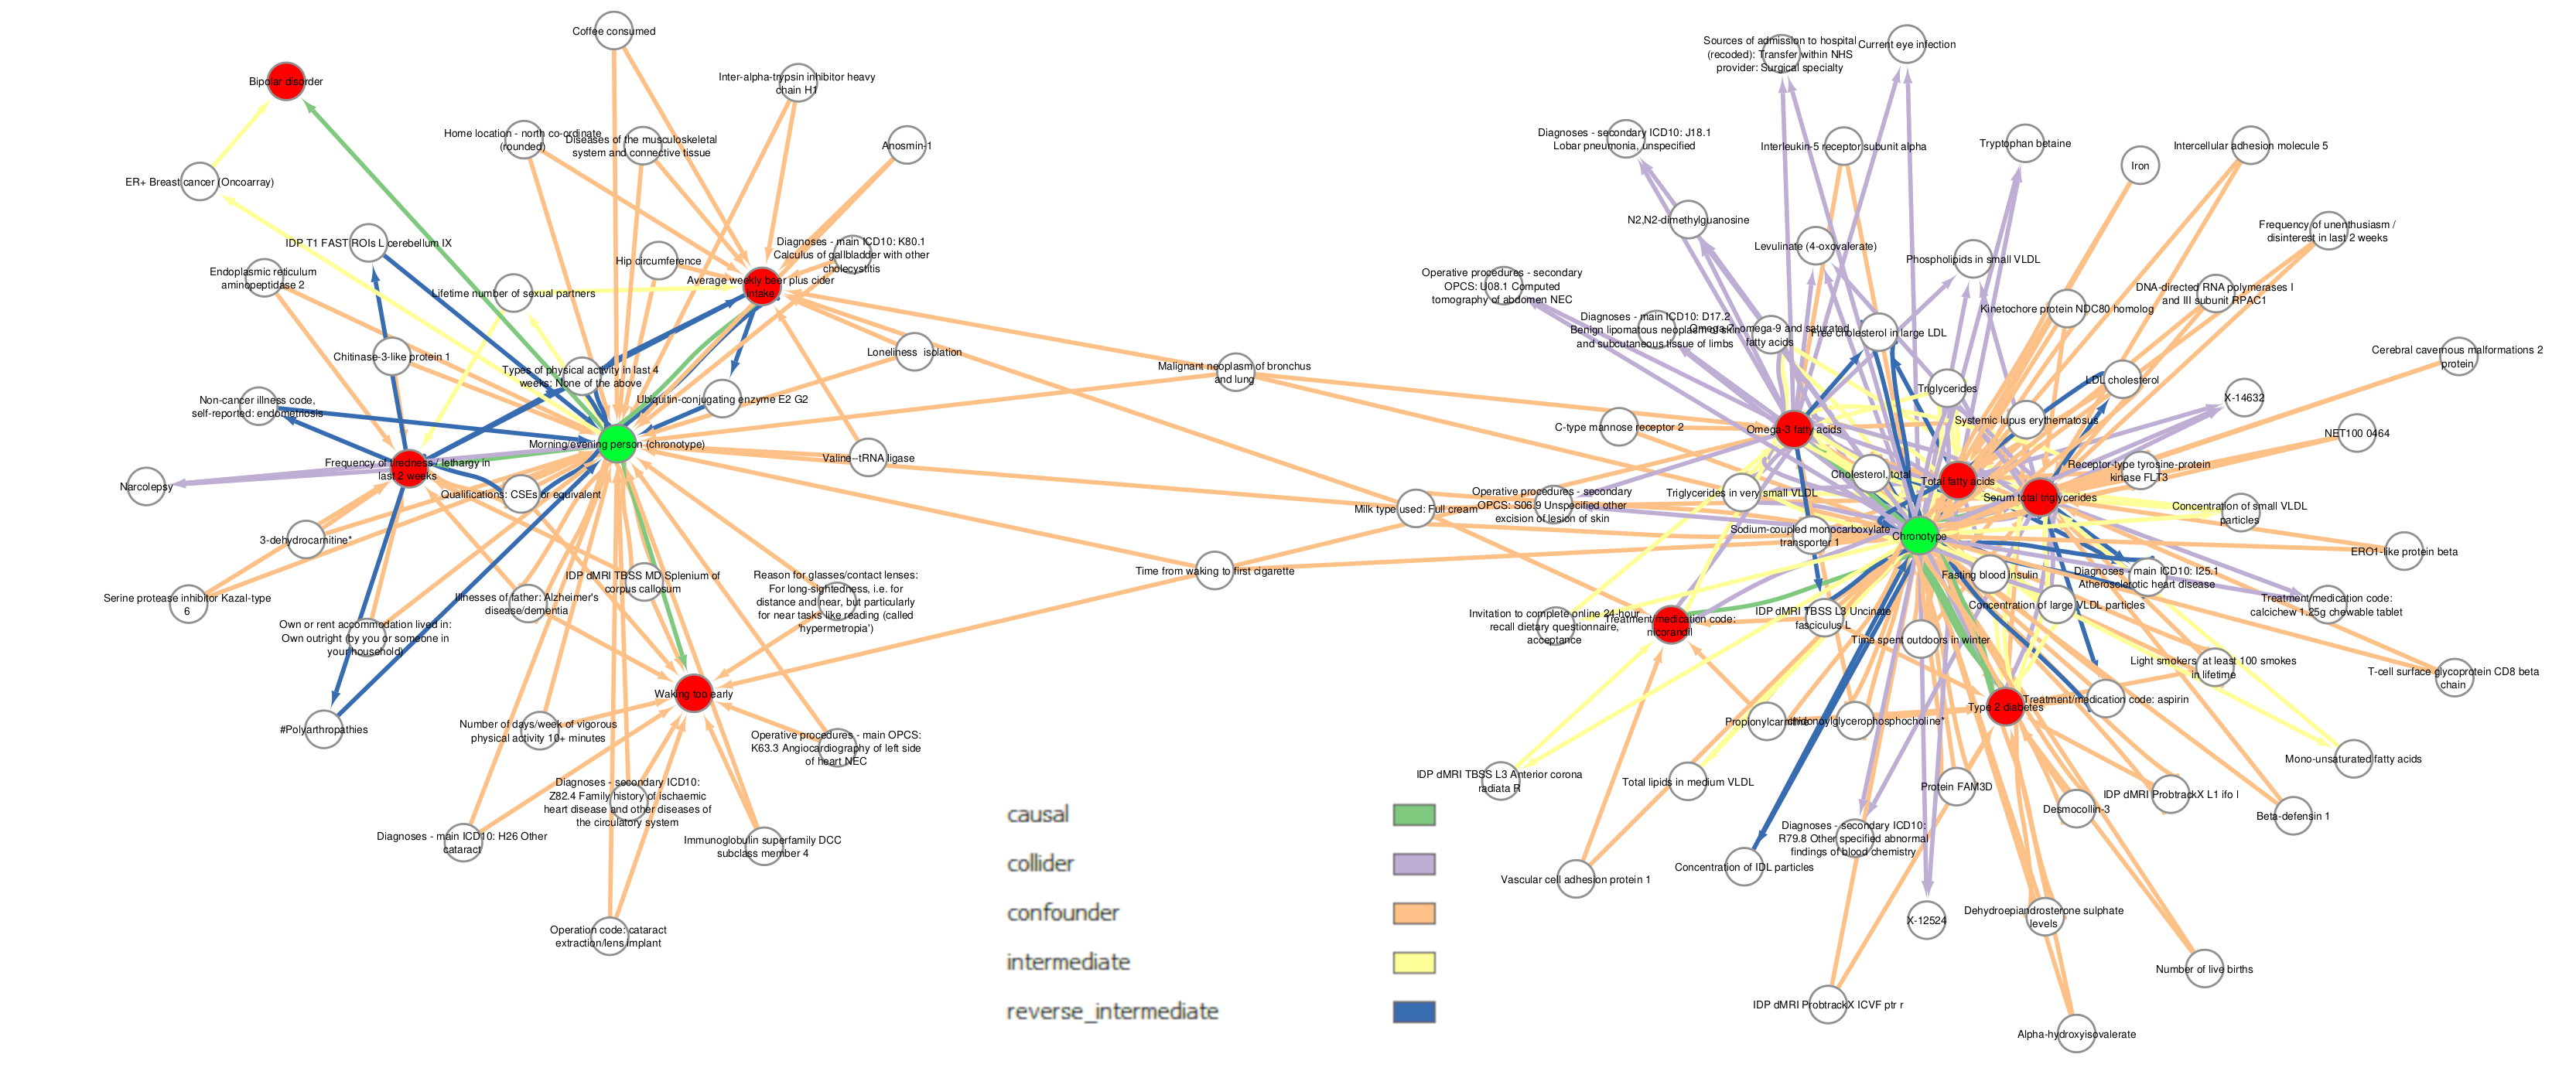
\includegraphics[width=\linewidth,keepaspectratio]{Figs/Analysis3/gBig.png}
\caption{Causal and confounding relationships between chronotype exposures (green nodes) and traits (red nodes). White nodes and potential confounding variables. Edges indicate the direction of causality (arrows). Green edges = causal relationships; Lavender = colliders, orange = confounders, yellow = intermediates, blue = reverse intermediates.}
\label{gBig}
%\end{subfigure}\\[1ex]
\end{sidewaysfigure}[htbp]



Not all MR analyses are beset by confounders, however. The relationship between exposure to an evening chronotype and bipolar disorder was not found to be influenced by a statistically significant confounder or collider. In addition to the direct relationship between chronotype and bipolar disorder, a mediator of the odds of ER+ breast cancer was discovered, see Figure~\ref{chronoBipolar}. The relationship from chronotype to cancer ($\beta$ 0.32) was stronger than the unmediated relationship directly to bipolar ($\beta$ 0.17), but weaker than the possible relationship of breast cancer to bipolar disorder ($\beta$ 0.42). 

As a last example study, the relationship between exposure to an evening chronotype and an increase of beer/wine intake was explored. There is a possible bi-directional relationship between chronotype and beer/alcohol intake, mediated by reverse-intermediates of a lack of physical activity (types of physical activity in the last 4 weeks: none of the above) and concentration of UBE2G2. Additionally, direct intermediates include the lifetime number of sexual partners. No colliders were present, but several potential confounders were identified which may need to be conditioned on, depending on study design. These included dietary consumption (milk type and coffee consumed), loneliness and isolation, hip circumference, and other metabolite measures. See Figure~\ref{chronoBeer}.

\begin{figure}[htbp]
\begin{subfigure}{.5\linewidth}
\centering
	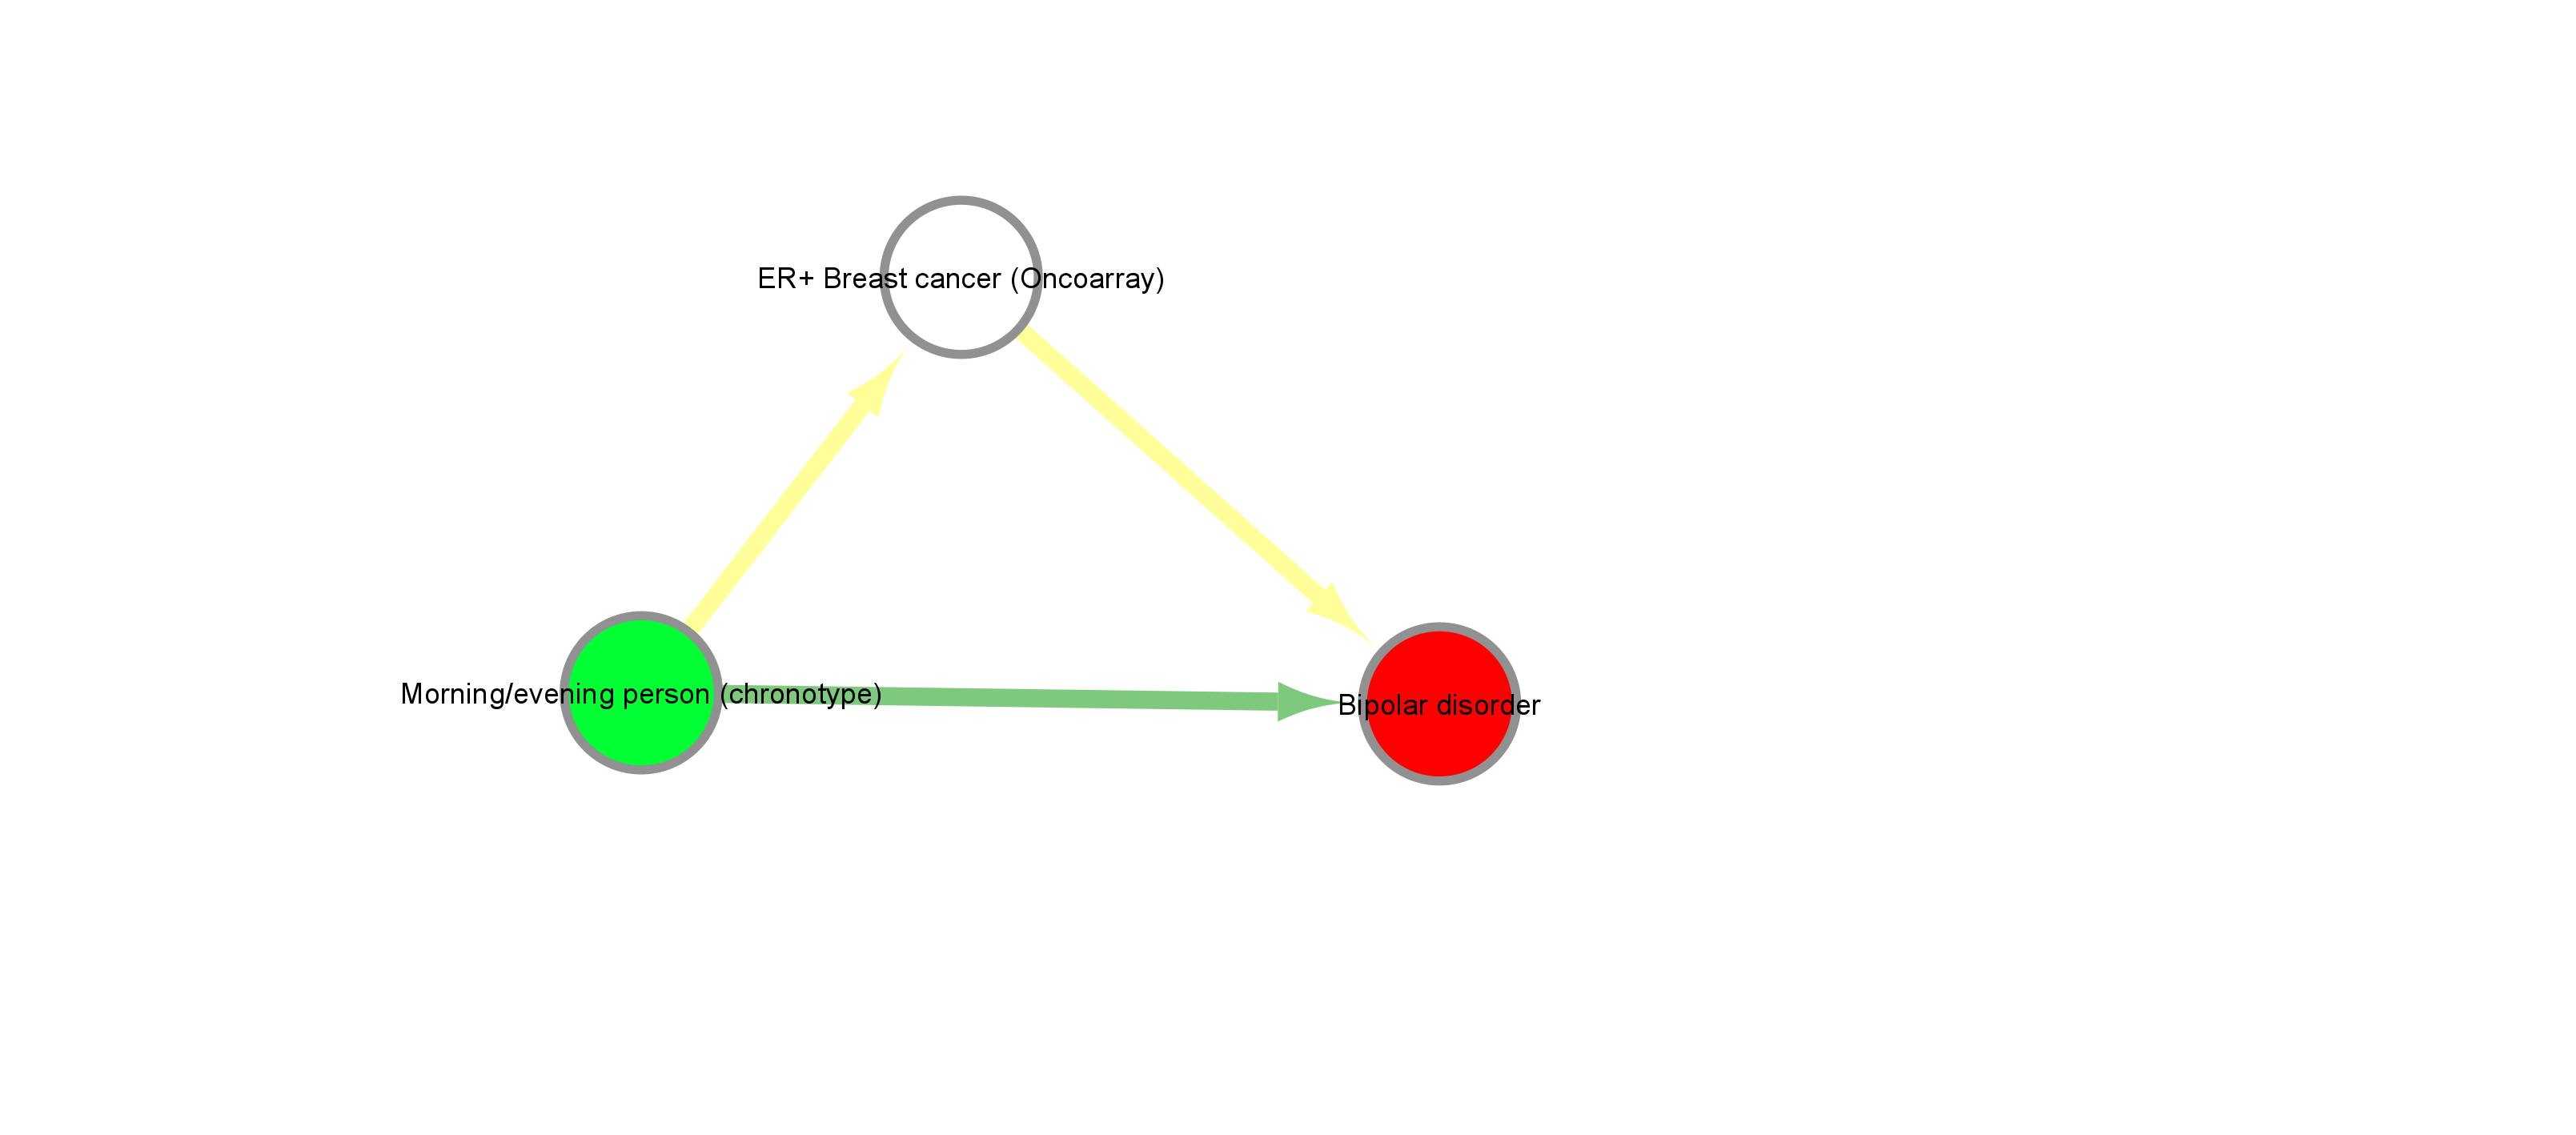
\includegraphics[width=0.9\linewidth,keepaspectratio]{Figs/Analysis3/morning_bipolar.png}
\caption{}
\label{chronoBipolar}
\end{subfigure}
\begin{subfigure}{.5\linewidth}
\centering
	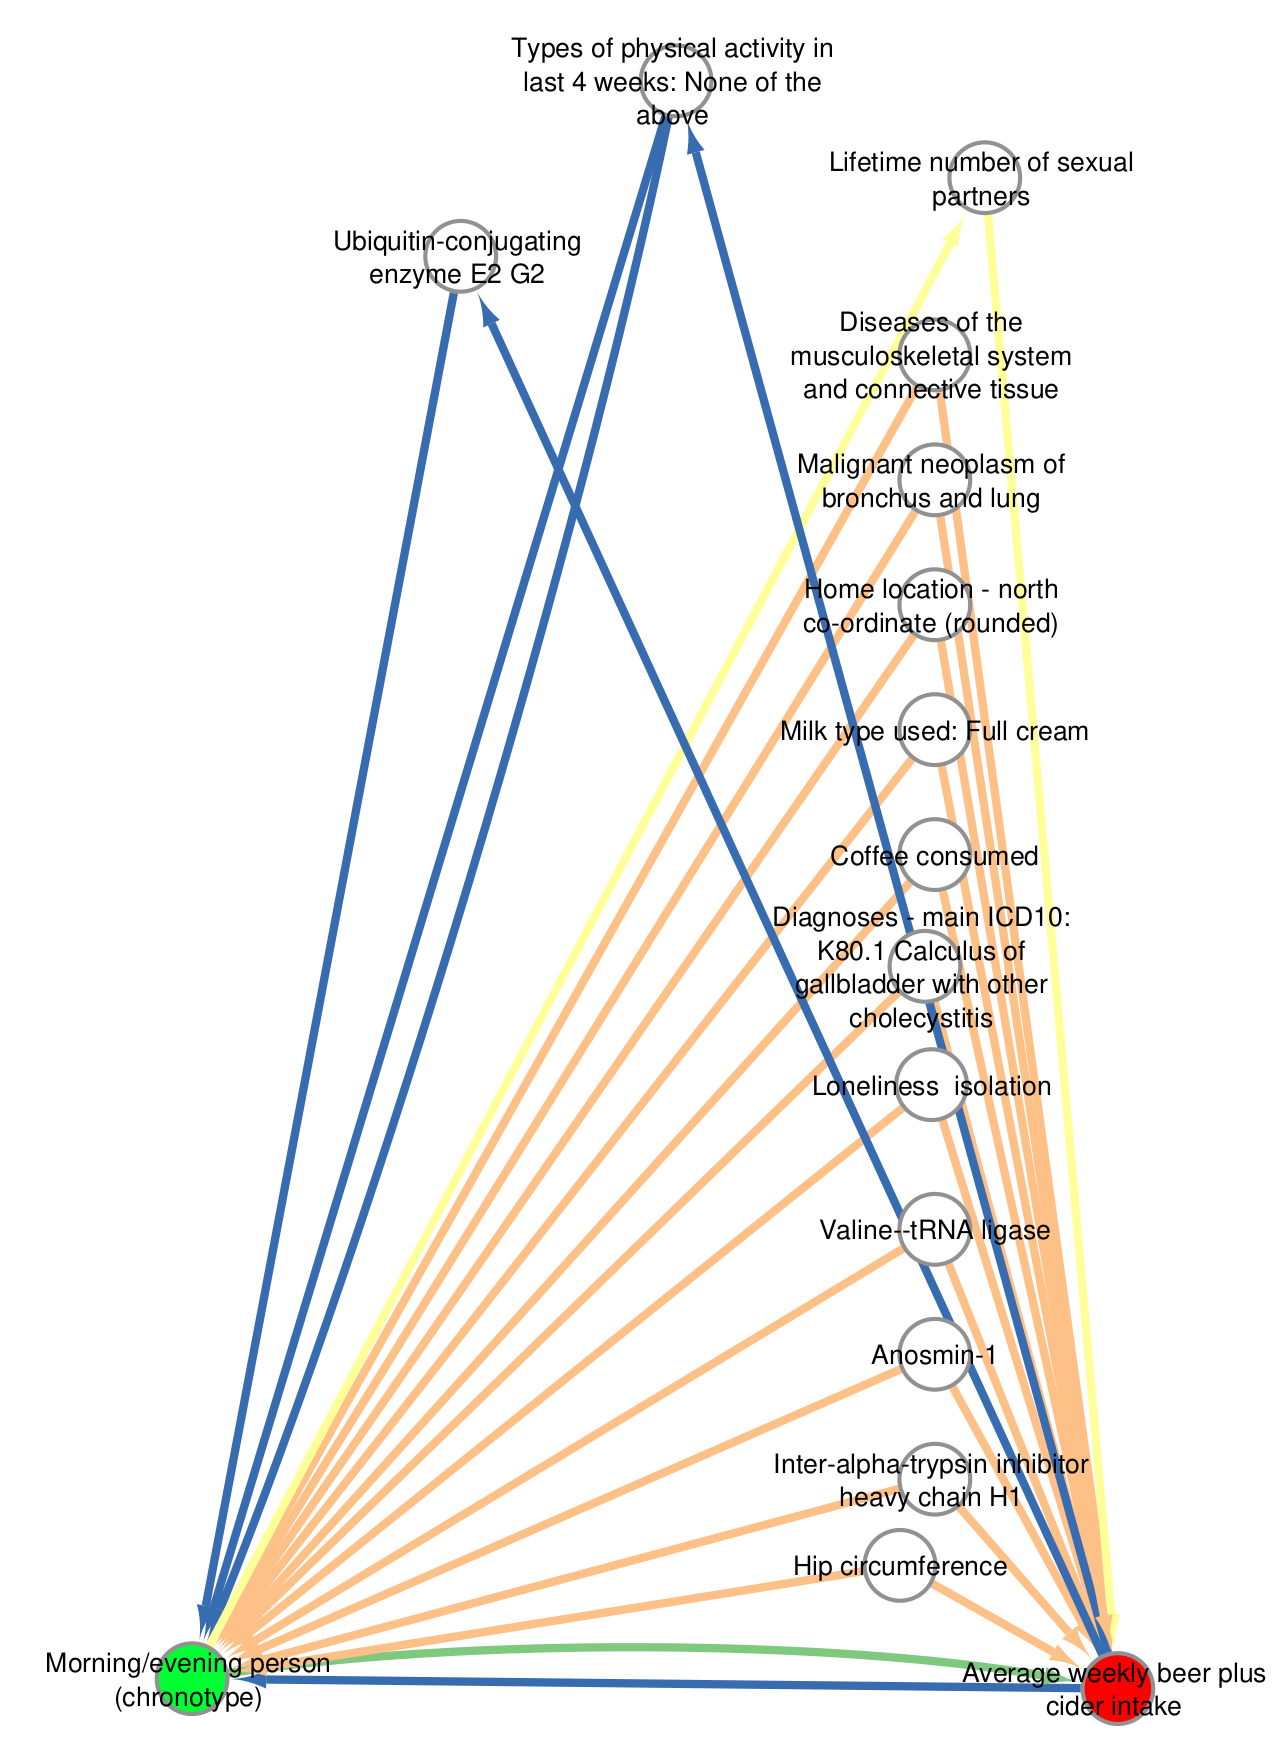
\includegraphics[width=0.9\linewidth,keepaspectratio]{Figs/Analysis3/chronoBeer.png}
\caption{}
\label{chronoBeer}
\end{subfigure}
\caption{(a) An evening chronotype associates with bipolar disorder. In addition to a valid association between chronotype and bipolar disorder, an intermediate association (p < 1e-5) was found for ER+ breast cancer. (b) An evening chronotype associates with increased beer and cider consumption. There is a potential bi-directional relationship between increased alcohol intake and an evening chronotype both directly (blue lines) and mediated by lack of physical activity and elevated UBE2G2. Chronotype may influence the number of sexual partners, which may influence average alcohol intake (yellow). There are numerous potential confounders relating body composition, loneliness, and diet.}
\label{chronoBeerBipolar}
\end{figure}




%%%%%%%%%%%%%%%%%%%%%%%%%%%%%%%%%%%%%%%%%%
\section{Discussion}

% group analyses (analysis A)
This analysis characterised the influence of an evening chronotype on cardiometabolic and behavioral traits. Chronotype, a measure of circadian rhythm, is a largely endogenous process though there are sustaining queues, zeitgebers, which influence chronotype \cite{albrecht_timing_2012}. The translational importance of understanding circadian biology is not limited to neurobehavioral function; the interplay between metabolism and circadian biology has been highlighted heavily in recent years. The gut microbiome, adipose cytokines, and metabolic hormones from ghrelin to leptin are all strongly regulated by circadian biology \cite{li_circadian_2020,socaciu_melatonin_2020,pan_circadian_2020}. Recent Mendelian randomization studies have also suggested a strong causal link between chronotype (a gross circadian phenotype) and body composition, free fatty acid circulation, and adiposity \cite{adams_evaluating_2019,jones_genome-wide_2019}. The current analysis revealed strong associations between chronotype and 10 other biological traits. In Figure~\ref{forestIVW}, we reproduced causal associations between diabetes and triglycerides. Additionally, we report novel associations by between chronotype and metabolomic data (Omega-3 fatty acids, total faddy acids, Bilirubin). The strongest signals include diabetes and bipolar disorder, highlighting chronotype as a link between metabolic and psychiatric health. While not all IVW MR studies passed multiple testing correction, those that did had complex relationships with other traits, various degrees of heterogeneity and potential interplay in horizontal pleiotropy.
% individual analyses (analysis B)
All serum triglyceride associations and a link to type-2 diabetes had the same relationship to chronotype: increased risk or concentration of the trait on an exposure to a genetic predisposition to eveningness. Interestingly, there was a significant (albeit small) association between eveningness and a decrease in likelihood to be taking nicorandil, a ventilator used to treat angina (see Figure~\ref{nicorandil}. Nicorandil has been shown in one study to affect the diurnal rhythms in body temperature and heart rate in rats \cite{Gantenbein}. There is no evidence that the drug affects circadian behavior in humans, although variant angina (treated with nicorandil) has a circadian component, supporting the idea that the influence of circadian biology may contribute to some types of angina that are amenable to nicorandil treatment \cite{Kusama}. The influence of chronotype on alcohol consumption was recently investigated by Hisler and colleagues, who revealed a 24 hour rhythm of alcohol craving in late adolescent adults and showed that an evening chronotype corresponds to a later craving for alcohol \cite{Hisler}. The associations between an evening chronotype and bipolar disorder are well documented \cite{Ferrer}, and has been proposed as an endophenotype to classify subtypes of bipolar \cite{romo-nava}, though several interacting traits may play a role in these subtypes.
% confounder analyses (analysis C)
Not surprisingly, there were over 200 potential confounders or mediators observed between chronotype and the ten significant exposures studied. As evidenced by Figure~\ref{gBig}, they vary in type from acceptable in an MR analysis (intermediate, possibly reverse intermediate depending on follow-up studies) to those that must be conditioned upon to maintain causality (the most abundant intermediate, confounders) to the more problematic colliders. Colliders are so called because the causal arrows in a directed acyclic graph from exposure and outcome both impact (collide on) the variable. Unlike confounders, conditioning on colliders in regression introduces bias into the association between exposure and outcome \cite{Rohrer}. The four associations subject to collider bias are the relationship between chronotype and omega-3 fatty acids, serum total triglycerides, total fatty acids, and lethargy. Possible confounders for the three metabolites include other cardiometabolic parameters, including total fatty acids, fasting insulin, and VLDL concentrations. The release of metabolomic data in the UK Biobank \cite{biobank} caters for new opportunities to investigate these collisions experimentally since they relate to chronotype and both psychiatric and cardiometabolic diseases. The only collider associated to lethargy was narcolepsy, an intuitive yet potentially complex relationship. The only confounder between an evening chronotype found in this study was ER+ breast cancer. The confounding was as an intermediate, which maintains the causal nature of the analysis while adding an extra explanatory "path" to get from exposure to outcome. While there is no current literature directly linking chronotype to breast cancer and then to the presence of bipolar disorder, this may be investigated in current murine models of breast cancer via knockdown experiments or by manipulating light as an external zeitgeber.

% Phenome-wide approach and potential criticisms
Instrumental variable analysis relies on strong assumptions, and occasionally unverifiable conditions \cite{labrecqueUnderstandingAssumptionsUnderlying2018}. Subject knowledge is the most reliable method for concluding assumptions are valid, especially when choosing exposures and outcomes correctly. A naive, phenome-wide search for causation between traits is likely to include among many tests non-plausible experimental designs, leading to an artificial increase in multiple testing burden and design flaws. This is evident by the need to prune associations in the first step of this study. In our re-analysis of traits in step 2, we failed to replicate the extremely low p-values present in the EpiGraphDB, even when using the same outcome and exposure studies obtained by a sister database, MR-Base. Without access to the underlying filtering methods used in the large repositories, we can speculate that instrumental variable selection, LD clumping, and filtering played a part. However, this re-analysis has produced associations that stand up to multiple testing while revealing novel associations. This study was limited to viewing causality through the lens of Mendelian Randomization alone. In our previous work, we have used gene expression data to identify causal regulatory networks using Bayesian approaches \cite{Aziz_2020}. Opportunities exist to combine these approaches, creating multimodal graphs of gene regulatory networks from that approach with the multi-trait networks created in this work. 

%%%%%%%%%%%%%%%%%%%%%%%%%%%%%%%%%%%%%%%%%%
\section{Conclusions}
Our findings have revealed potential causal associations between chronotype and several behavioral and metabolic traits. While using publicly available data to confirm previously known associations (T2DM, cholesterol) we have found novel associations which may be validated experimentally in models. These include associations between chronotype and the vasodilator Nicorandil, and a relationship between chronotype and bipolar disorder potentially mediated by estrogen-receptive breast cancer. Lastly, we have revealed potential confounders and colliders impacting the relationship between chronotype and commonly reported cardiometabolic traits which should be addressed through a combination of multivariate and multi-stage analyses as appropriate.


%%%%%%%%%%%%%%%%%%%%%%%%%%%%%%%%%%%%%%%%%%
% \section{Patents}

% This section is not mandatory, but may be added if there are patents resulting from the work reported in this manuscript.

%%%%%%%%%%%%%%%%%%%%%%%%%%%%%%%%%%%%%%%%%%
\vspace{6pt} 

%%%%%%%%%%%%%%%%%%%%%%%%%%%%%%%%%%%%%%%%%%
%% optional
%\supplementary{The following are available online at \linksupplementary{s1}, Figure S1: title, Table S1: title, Video S1: title.}

% Only for the journal Methods and Protocols:
% If you wish to submit a video article, please do so with any other supplementary material.
% \supplementary{The following are available at \linksupplementary{s1}, Figure S1: title, Table S1: title, Video S1: title. A supporting video article is available at doi: link.} 

%%%%%%%%%%%%%%%%%%%%%%%%%%%%%%%%%%%%%%%%%%
\authorcontributions{\authorcontributions{Conceptualization, J.A.W.; methodology, J.A.W.; software, J.A.W; validation J.A.W.; formal analysis J.A.W.; investigation, J.A.W., D.R., V.R.C., L.B.M., S.P., F.A., A.A., G.V.G.; writing–original draft preparation, J.A.W, G.V.G; writing–review and editing,J.A.W., D.R., V.R.C., L.B.M., S.P., F.A., A.A., G.V.G.; visualization, J.A.W.; supervision, A.A., G.V.G; project administration, G.V.G; funding acquisition, G.V.G.}}
%For research articles with several authors, a short paragraph specifying their individual contributions must be provided. The following statements should be used ``Conceptualization, X.X. and Y.Y.; methodology, X.X.; software, X.X.; validation, X.X., Y.Y. and Z.Z.; formal analysis, X.X.; investigation, X.X.; resources, X.X.; data curation, X.X.; writing---original draft preparation, X.X.; writing---review and editing, X.X.; visualization, X.X.; supervision, X.X.; project administration, X.X.; funding acquisition, Y.Y. All authors have read and agreed to the published version of the manuscript.'', please turn to the  \href{http://img.mdpi.org/data/contributor-role-instruction.pdf}{CRediT taxonomy} for the term explanation. Authorship must be limited to those who have contributed substantially to the work~reported.}

\funding{The authors acknowledge support from the NIHR Birmingham ECMC, NIHR Birmingham SRMRC, Nanocommons H2020-EU (731032) and the NIHR Birmingham Biomedical Research Centre and the MRC Heath Data Research UK (HDRUK/CFC/01), an initiative funded by UK Research and Innovation, Department of Health and Social Care (England) and the devolved administrations, and leading medical research charities. The views expressed in this publication are those of the authors and not necessarily those of the NHS, the National Institute for Health Research, the Medical Research Council or the Department of Health.}

%\institutionalreview{In this section, please add the Institutional Review Board Statement and approval number for studies involving humans or animals. Please note that the Editorial Office might ask you for further information. Please add ``The study was conducted according to the guidelines of the Declaration of Helsinki, and approved by the Institutional Review Board (or Ethics Committee) of NAME OF INSTITUTE (protocol code XXX and date of approval).'' OR ``Ethical review and approval were waived for this study, due to REASON (please provide a detailed justification).'' OR ``Not applicable'' for studies not involving humans or animals. You might also choose to exclude this statement if the study did not involve humans or animals.}

%\informedconsent{Any research article describing a study involving humans should contain this statement. Please add ``Informed consent was obtained from all subjects involved in the study.'' OR ``Patient consent was waived due to REASON (please provide a detailed justification).'' OR ``Not applicable'' for studies not involving humans. You might also choose to exclude this statement if the study did not involve humans.

%Written informed consent for publication must be obtained from participating patients who can be identified (including by the patients themselves). Please state ``Written informed consent has been obtained from the patient(s) to publish this paper'' if applicable.}

\dataavailability{Data are available via the EpiGraphDB and MRBase APIs.} 

%\acknowledgments{In this section you can acknowledge any support given which is not covered by the author contribution or funding sections. This may include administrative and technical support, or donations in kind (e.g., materials used for experiments).}

\conflictsofinterest{The authors declare no conflict of interest.} 

%% Optional
%\sampleavailability{Samples of the compounds ... are available from the authors.}

%%%%%%%%%%%%%%%%%%%%%%%%%%%%%%%%%%%%%%%%%%
%% Only for journal Encyclopedia
%\entrylink{The Link to this entry published on the encyclopedia platform.}

%%%%%%%%%%%%%%%%%%%%%%%%%%%%%%%%%%%%%%%%%%
%% Optional
\abbreviations{The following abbreviations are used in this manuscript:\\

\noindent 
\begin{tabular}{@{}ll}
MDPI & Multidisciplinary Digital Publishing Institute\\
DOAJ & Directory of open access journals\\
TLA & Three letter acronym\\
LD & Linear dichroism
\end{tabular}}

%%%%%%%%%%%%%%%%%%%%%%%%%%%%%%%%%%%%%%%%%%
%% Optional
% \appendixtitles{no} % Leave argument "no" if all appendix headings stay EMPTY (then no dot is printed after "Appendix A"). If the appendix sections contain a heading then change the argument to "yes".
% \appendixstart
% \appendix
% \section{}
% \subsection{}
% The appendix is an optional section that can contain details and data supplemental to the main text---for example, explanations of experimental details that would disrupt the flow of the main text but nonetheless remain crucial to understanding and reproducing the research shown; figures of replicates for experiments of which representative data are shown in the main text can be added here if brief, or as Supplementary Data. Mathematical proofs of results not central to the paper can be added as an appendix.

% \begin{specialtable}[H] 
% %\tablesize{\scriptsize}
% \caption{This is a table caption. Tables should be placed in the main text near to the first time they are~cited.\label{tab1}}
% %\tablesize{} % You can specify the fontsize here, e.g., \tablesize{\footnotesize}. If commented out \small will be used.
% \begin{tabular}{ccc}
% \toprule
% \textbf{Title 1}	& \textbf{Title 2}	& \textbf{Title 3}\\
% \midrule
% Entry 1		& Data			& Data\\
% Entry 2		& Data			& Data\\
% \bottomrule
% \end{tabular}
% \end{specialtable}

% \section{}
% All appendix sections must be cited in the main text. In the appendices, Figures, Tables, etc. should be labeled, starting with ``A''---e.g., Figure A1, Figure A2, etc. 

%%%%%%%%%%%%%%%%%%%%%%%%%%%%%%%%%%%%%%%%%%
%\end{paracol}
\reftitle{References}

% Please provide either the correct journal abbreviation (e.g. according to the “List of Title Word Abbreviations” http://www.issn.org/services/online-services/access-to-the-ltwa/) or the full name of the journal.
% Citations and References in Supplementary files are permitted provided that they also appear in the reference list here. 

%=====================================
% References, variant A: external bibliography
%=====================================
\externalbibliography{yes}
\bibliography{references}

%=====================================
% References, variant B: internal bibliography
%=====================================
% \begin{thebibliography}{999}
% % Reference 1
% \bibitem[Author1(year)]{ref-journal}
% Author~1, T. The title of the cited article. {\em Journal Abbreviation} {\bf 2008}, {\em 10}, 142--149.
% % Reference 2
% \bibitem[Author2(year)]{ref-book1}
% Author~2, L. The title of the cited contribution. In {\em The Book Title}; Editor1, F., Editor2, A., Eds.; Publishing House: City, Country, 2007; pp. 32--58.
% % Reference 3
% \bibitem[Author3(year)]{ref-book2}
% Author 1, A.; Author 2, B. \textit{Book Title}, 3rd ed.; Publisher: Publisher Location, Country, 2008; pp. 154--196.
% % Reference 4
% \bibitem[Author4(year)]{ref-unpublish}
% Author 1, A.B.; Author 2, C. Title of Unpublished Work. \textit{Abbreviated Journal Name} stage of publication (under review; accepted; in~press).
% % Reference 5
% \bibitem[Author5(year)]{ref-communication}
% Author 1, A.B. (University, City, State, Country); Author 2, C. (Institute, City, State, Country). Personal communication, 2012.
% % Reference 6
% \bibitem[Author6(year)]{ref-proceeding}
% Author 1, A.B.; Author 2, C.D.; Author 3, E.F. Title of Presentation. In Title of the Collected Work (if available), Proceedings of the Name of the Conference, Location of Conference, Country, Date of Conference; Editor 1, Editor 2, Eds. (if available); Publisher: City, Country, Year (if available); Abstract Number (optional), Pagination (optional).
% % Reference 7
% \bibitem[Author7(year)]{ref-thesis}
% Author 1, A.B. Title of Thesis. Level of Thesis, Degree-Granting University, Location of University, Date of Completion.
% % Reference 8
% \bibitem[Author8(year)]{ref-url}
% Title of Site. Available online: URL (accessed on Day Month Year).
% \end{thebibliography}

% If authors have biography, please use the format below
%\section*{Short Biography of Authors}
%\bio
%{\raisebox{-0.35cm}{\includegraphics[width=3.5cm,height=5.3cm,clip,keepaspectratio]{Definitions/author1.pdf}}}
%{\textbf{Firstname Lastname} Biography of first author}
%
%\bio
%{\raisebox{-0.35cm}{\includegraphics[width=3.5cm,height=5.3cm,clip,keepaspectratio]{Definitions/author2.jpg}}}
%{\textbf{Firstname Lastname} Biography of second author}

% The following MDPI journals use author-date citation: Arts, Econometrics, Economies, Genealogy, Humanities, IJFS, JRFM, Laws, Religions, Risks, Social Sciences. For those journals, please follow the formatting guidelines on http://www.mdpi.com/authors/references
% To cite two works by the same author: \citeauthor{ref-journal-1a} (\citeyear{ref-journal-1a}, \citeyear{ref-journal-1b}). This produces: Whittaker (1967, 1975)
% To cite two works by the same author with specific pages: \citeauthor{ref-journal-3a} (\citeyear{ref-journal-3a}, p. 328; \citeyear{ref-journal-3b}, p.475). This produces: Wong (1999, p. 328; 2000, p. 475)

%%%%%%%%%%%%%%%%%%%%%%%%%%%%%%%%%%%%%%%%%%
%% for journal Sci
%\reviewreports{\\
%Reviewer 1 comments and authors’ response\\
%Reviewer 2 comments and authors’ response\\
%Reviewer 3 comments and authors’ response
%}
%%%%%%%%%%%%%%%%%%%%%%%%%%%%%%%%%%%%%%%%%%
\end{document}

